\documentclass[12pt,a4paper,oneside]{report}

%Options: Sonny, Lenny, Glenn, Conny, Rejne, Bjarne, Bjornstrup
%\usepackage[Lenny]{fncychap}
\usepackage{graphicx}
\usepackage{float}
%\usepackage[top=2cm, bottom=2cm, left=1in, right=2cm]{geometry}
\usepackage[margin=1in]{geometry}
\usepackage[T1]{fontenc}
\usepackage[utf8]{inputenc}
\usepackage{mwe}
\usepackage{fancyhdr}

\usepackage{amsthm}
\usepackage{amsfonts}
\usepackage{amssymb}
\usepackage{amsmath}
\usepackage{fourier}

% Make TOC clickable link
\usepackage{hyperref}
\hypersetup{
    colorlinks,
    citecolor=black,
    filecolor=black,
    linkcolor=black,
    urlcolor=black
}

\usepackage{multicol}
\usepackage{caption}
\usepackage[percent]{overpic}
\usepackage{xcolor} % For setting text color

% Add section title at the top of the page
\pagestyle{fancy}
\fancyhf{}
\fancyhead[L]{\rightmark}
\fancyhead[R]{\thepage}
\renewcommand{\headrulewidth}{0pt}

% To append pdf pages
\usepackage{pdfpages}

% line between column
\setlength{\columnseprule}{0.4pt}

%\titleformat{\chapter}[hang]{\Huge\bfseries}{\thechapter\hsp\textcolor{gray75}{|}\hsp}{0pt}{\Huge\bfseries}

%----------------COMMANDS-------------------------------------------%%
\newcommand\blank{\underline{\hspace{2cm}}} % Gives a blank 
\newcounter{prob} % A new counter for current problem number
\setcounter{prob}{1} % Start the counter at the value 1
\newcommand\itm{
	\fbox{\textbf{\theprob}} \refstepcounter{prob}
} % Calls problem number
\newcommand{\problemans}[2]{
	\noindent
	\begin{minipage}[t]{\textwidth}\itm #1 \end{minipage}  
	\rotatebox{180}{\scriptsize{Ans: #2}}
	\vfill
} % An environment for a problem statement on or more lines
\newcommand{\problem}[1]{
	\noindent
	\begin{minipage}[t]{\textwidth}\itm #1 \end{minipage}  
	\vfill
} % An environment for a problem statement on or more lines
\newcommand{\pairofprobsans}[4]{
	\noindent
	\begin{minipage}[t]{0.5\textwidth}\itm #1 \end{minipage}
	\begin{minipage}[t]{0.5\textwidth}\itm #3 \end{minipage} 
	\begin{minipage}[t]{\textwidth}\rotatebox[origin=c]{180}{\parbox{\textwidth}{\scriptsize{\hfill Ans: #4\hfill Ans: #2}}}\end{minipage}
	
	\vfill
} % Fits two problems on a line
\newcommand{\pairofprobs}[2]{
	\noindent
	\begin{minipage}[t]{0.5\textwidth}\itm #1 \end{minipage} 
	\begin{minipage}[t]{0.45\textwidth}\itm #2 \end{minipage} 
	\vfill
} % Fits two problems on a line
\newcommand{\threeprobs}[3]{
	\noindent
	\begin{minipage}[t]{0.31\textwidth}\itm #1 \end{minipage} \hfill
	\begin{minipage}[t]{0.31\textwidth}\itm #2 \end{minipage} \hfill 
	\begin{minipage}[t]{0.31\textwidth}\itm #3 \end{minipage}
	\vfill
} % Fits three problems on a line
\newcounter{choice} % Counter for multiple choice problems 
\setcounter{choice}{1} % Start the counter at the value 1
\newcommand\achoice{
	(\alph{choice}) \stepcounter{choice}
} % Generates letter for multiple choice option
\newcommand{\answers}[5]{\vspace*{-7mm} 
	\begin{tabular}{l@{\hspace{1mm}}p{0.9\textwidth}}
		\achoice & #1 \\ \achoice & #2 \\ \achoice & #3 \\ 
		\achoice & #4 \\ \achoice & #5 \end{tabular}
	\setcounter{choice}{1}
} % Makes multiple-choice options 
%---------------------------------


%---------------------------------
% Make a note with box
\usepackage[most]{tcolorbox}

\newtcolorbox{myframe}[1][]{
	enhanced,
	arc=0pt,
	outer arc=0pt,
	colback=white,
	boxrule=0.8pt,
	#1
}

% example
%\begin{myframe}[width=30em,top=20pt,bottom=20pt,left=20pt,right=20pt,arc=10pt,auto outer arc]
%	I certify that the work presented in the dissertation is my own unless referenced.
%\end{myframe}
%---------------------------------




%---------------------------------
% Reset the counter for prob in a new section
\newcommand{\makenewpage}{\newpage\setcounter{prob}{1}}
%---------------------------------

%----
% Make mainmatter frontmatter work in report
\makeatletter

\newcommand\frontmatter{%
	\cleardoublepage
	%\@mainmatterfalse
	\pagenumbering{roman}}

\newcommand\mainmatter{%
	\cleardoublepage
	% \@mainmattertrue
	\pagenumbering{arabic}}

\newcommand\backmatter{%
	\if@openright
	\cleardoublepage
	\else
	\clearpage
	\fi
	% \@mainmatterfalse
}

\makeatother
%----

%--------------
% Option to include or not for 
% 1. past years questions.
% 2. scheme of works
%--------------
\newif\ifincludepastyears
\newif\ifincludesow
%--------------

%--------------
% Define a new command for QR codes with captions
% \qrfigure{<image path>}{<caption text>}
%-------------
\newcommand{\qrfigure}[2]{
  \begin{figure}[h!]
    \hfill % Pushes the figure to the right
    \begin{minipage}{0.2\textwidth} % Adjust the width to fit the QR image
      \centering
      \begin{overpic}[width=\textwidth]{#1}
        % Position the caption text within the QR code's padding at the bottom
        \put(14,1){\color{black}\footnotesize #2}
      \end{overpic}
    \end{minipage}
  \end{figure}
}

% format chapter title
\usepackage{titlesec, color}
\definecolor{gray75}{gray}{0.75}
\newcommand{\hsp}{\hspace{20pt}}
\titleformat{\chapter}[hang]{\Huge\bfseries}{\thechapter\hsp\textcolor{gray75}{|}\hsp}{0pt}{\Huge\bfseries}
\titlespacing*{\chapter}{0pt}{-50pt}{20pt}

% format section title
\titleformat{\section}{\normalfont\Large\bfseries}{\thesection}{1em}{}[{\titlerule[0.8pt]}]

% Disable indent on a new paragraph.
\parindent 0px


\title{Calculus I Workbook}
\author{Profesor Madya Ts. Dr. Rizauddin Saian\\
https://www.rizauddin.com
}
\date{2024}

\begin{document}

%front page
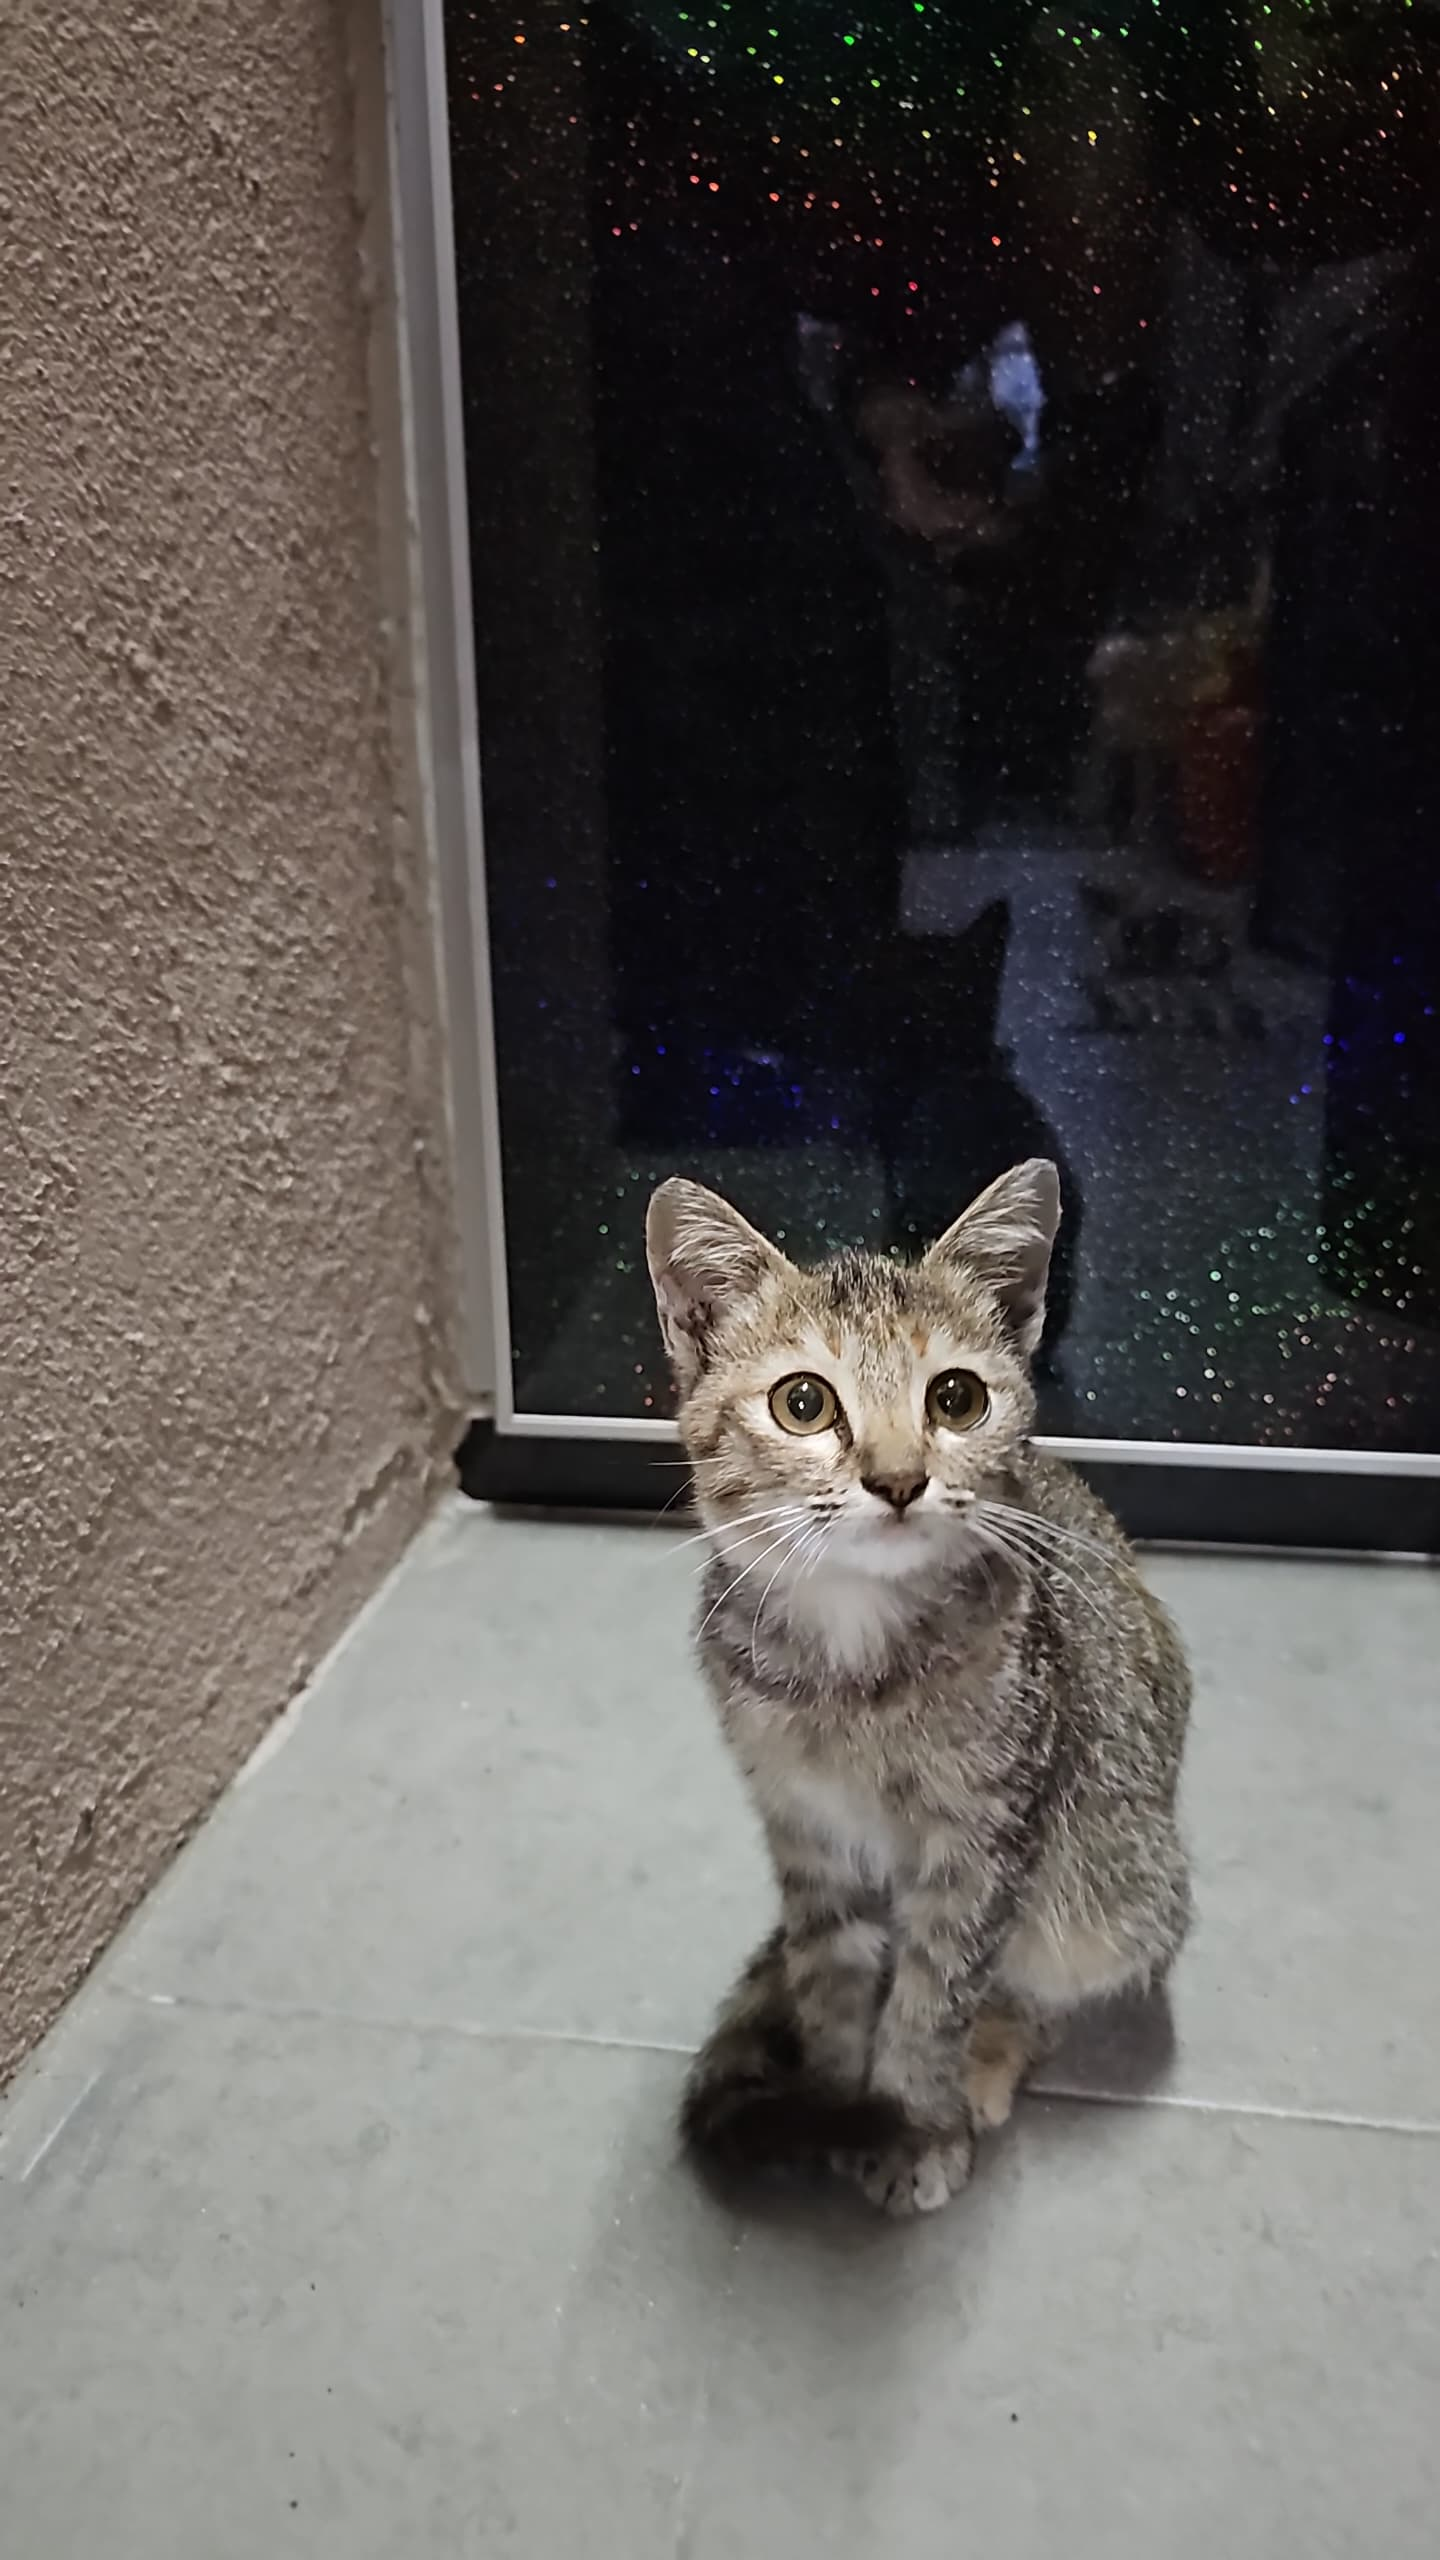
\includepdf[fitpaper=true, pages=-]{pdf/front2024}
%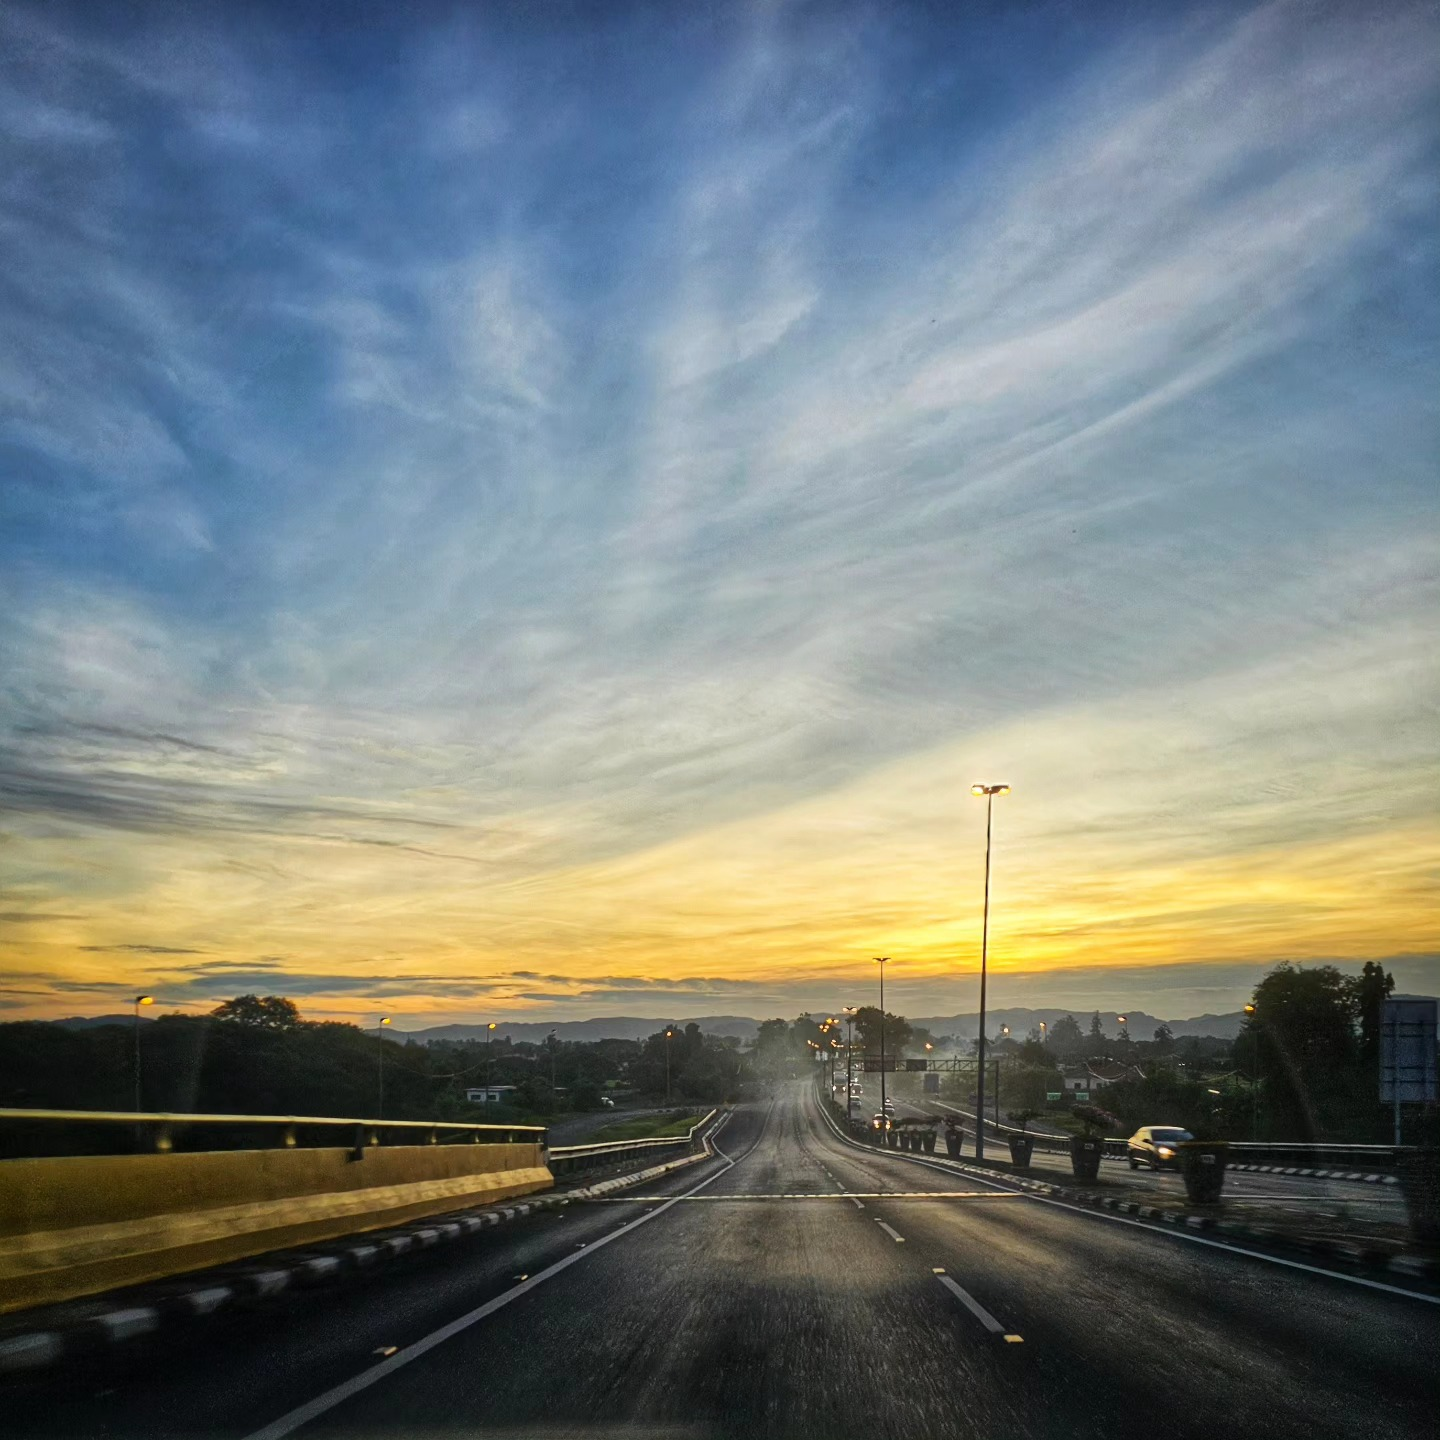
\includepdf[fitpaper=true, pages=-]{pdf/front}

\frontmatter

\maketitle

% scheme of works
%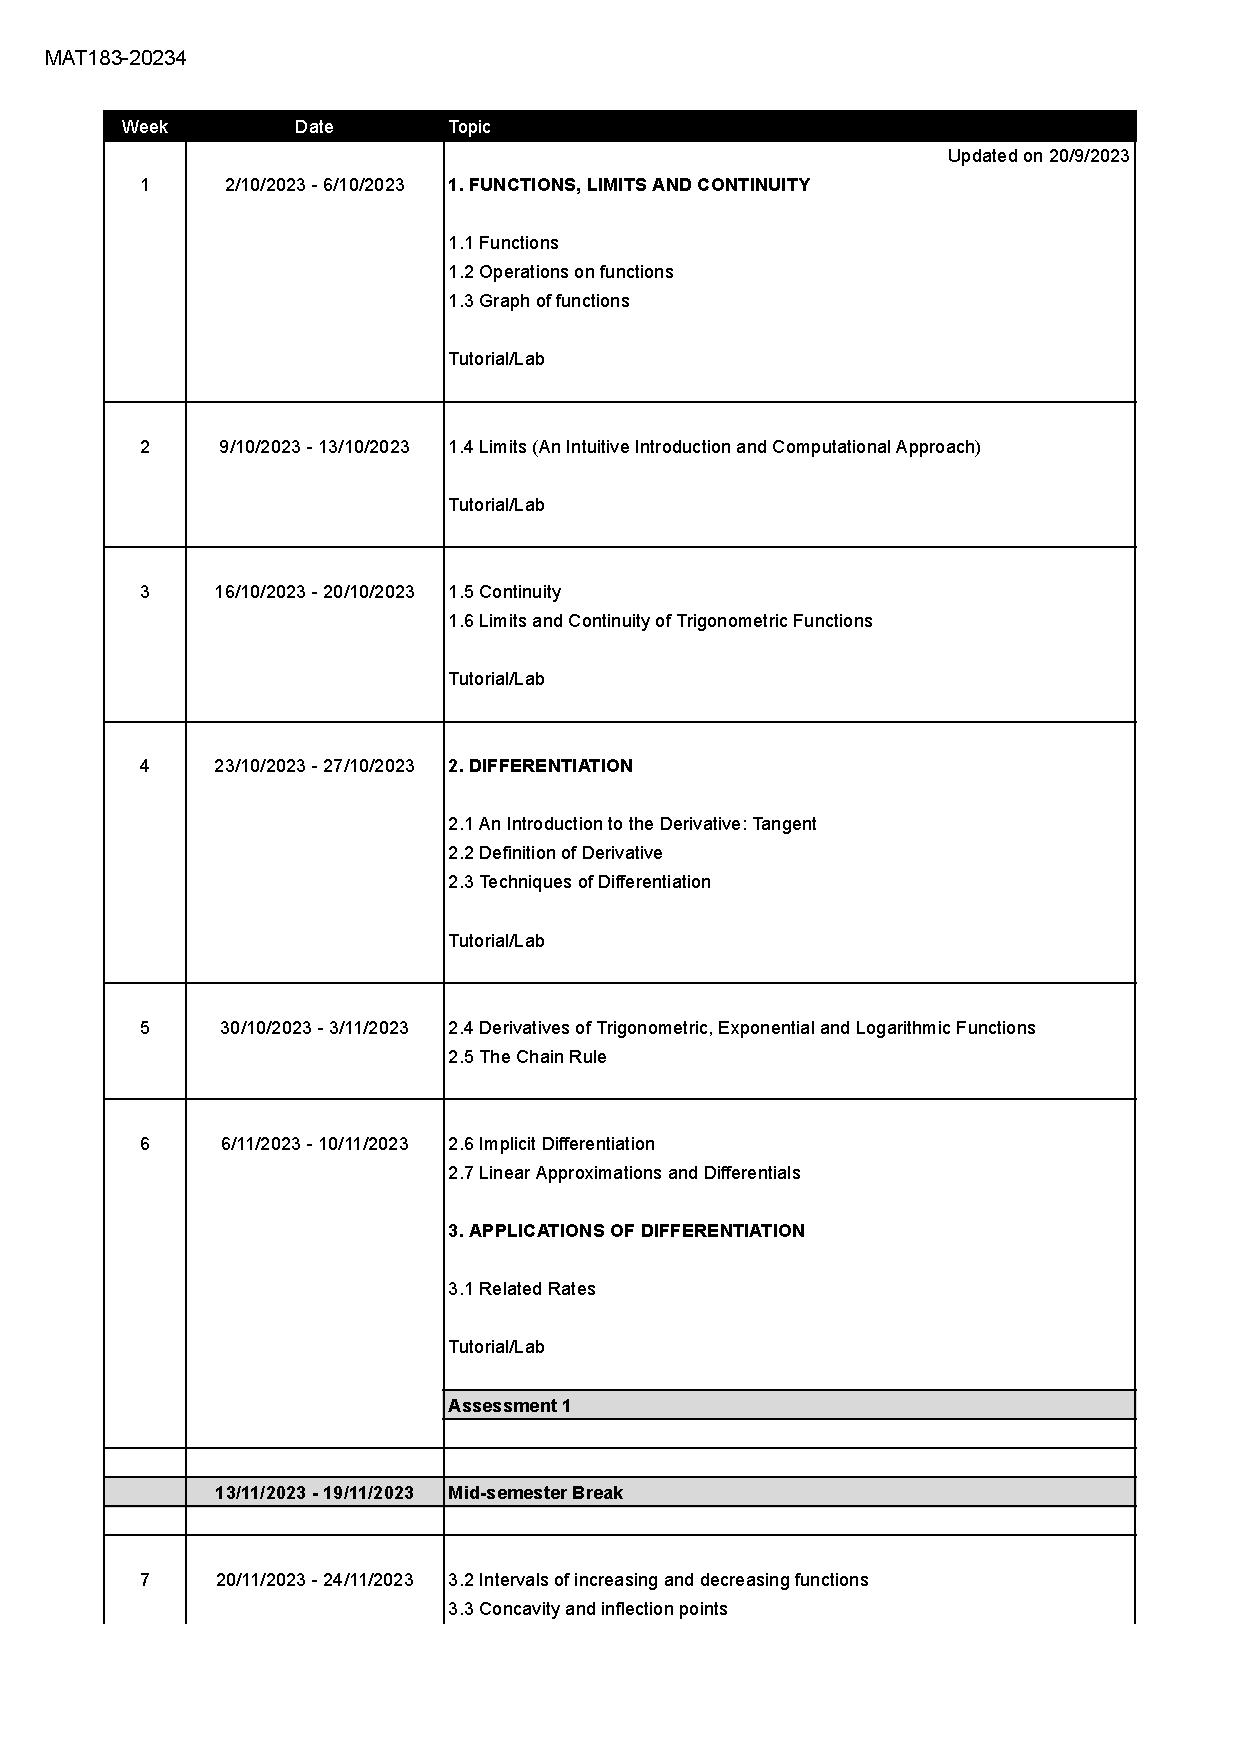
\includepdf[pages={1-},pagecommand={}]{pdf/MAT183-20234-SOW}
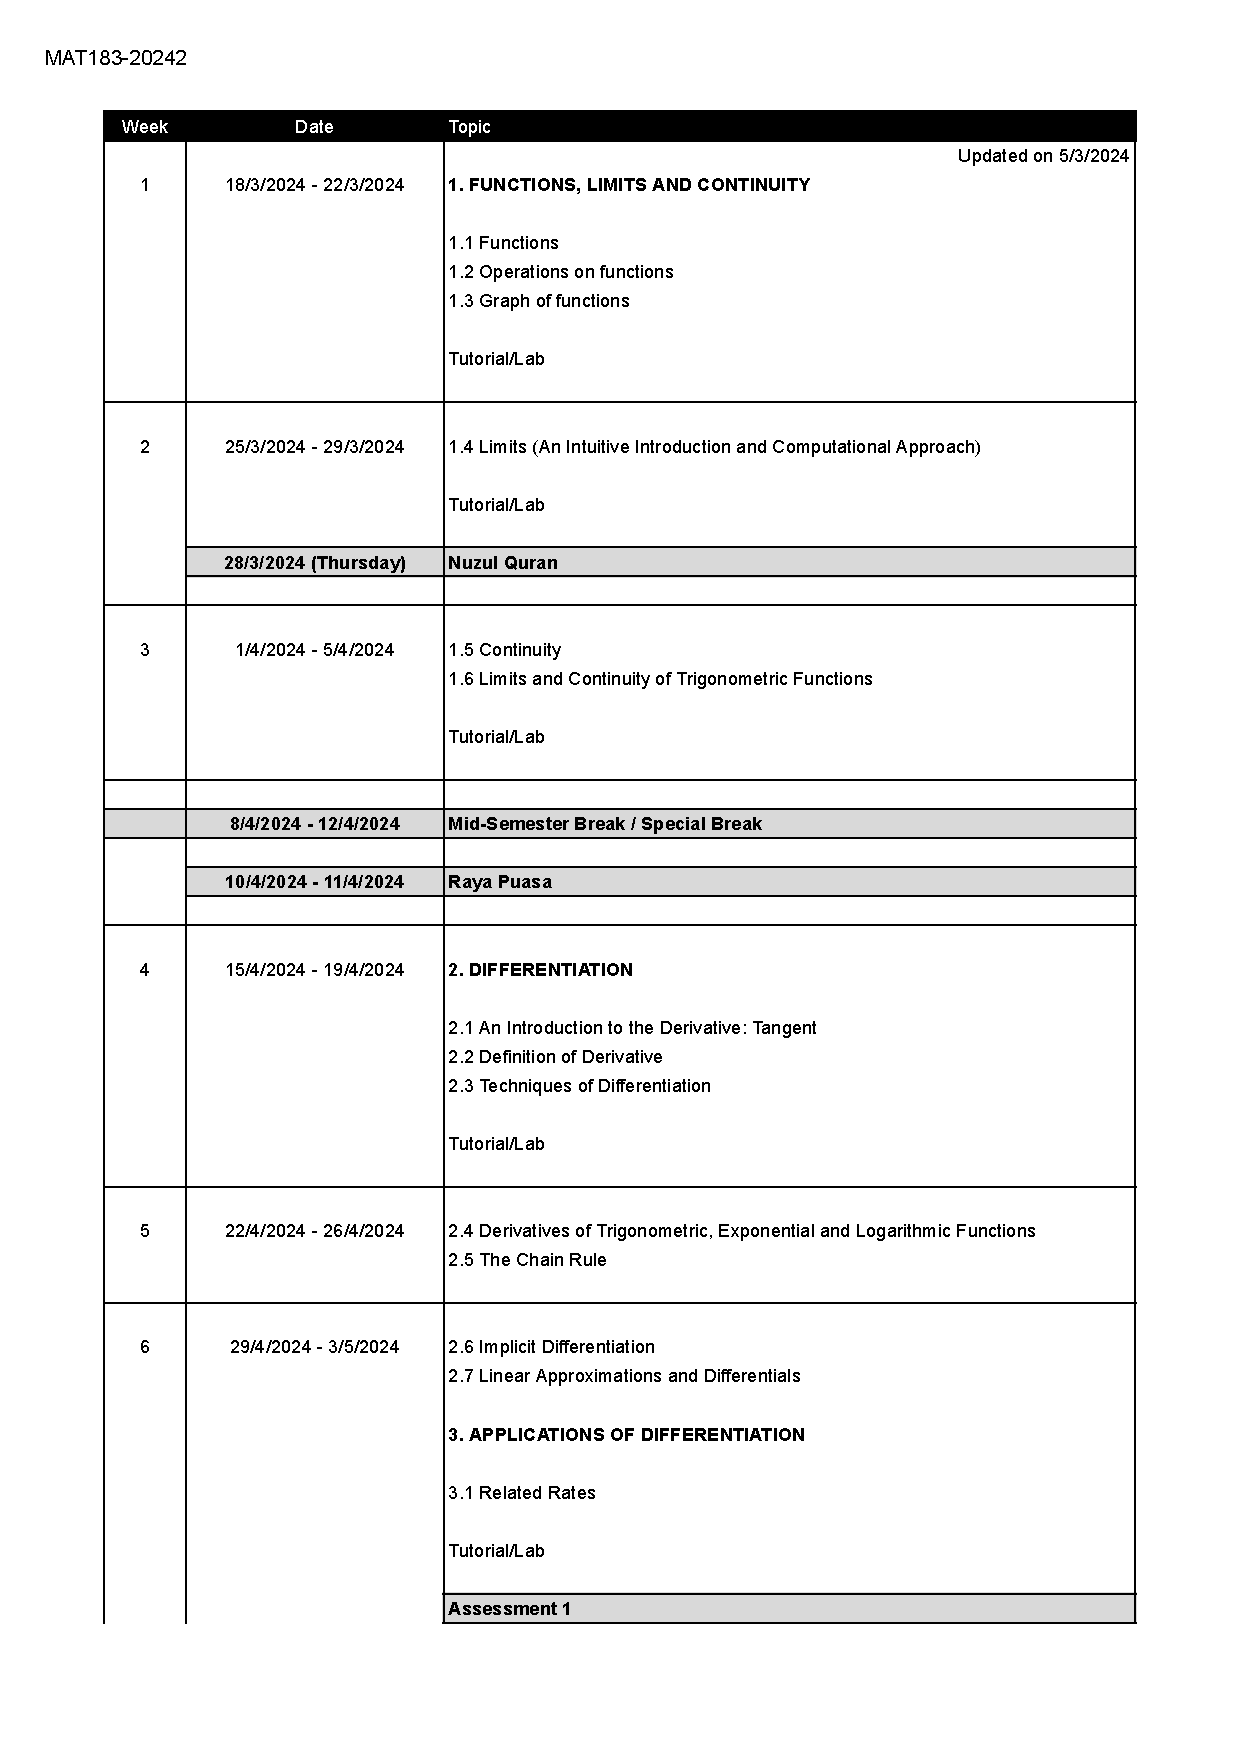
\includepdf[scale=0.8,pages={1},pagecommand={\chapter*{Scheme of Works}\addcontentsline{toc}{chapter}{Scheme of Works}}]{pdf/MAT183-20242-SOW}
\includepdf[scale=0.8,pages={2-},pagecommand={}]{pdf/MAT183-20242-SOW}

% preface
\chapter*{Preface}
\addcontentsline{toc}{chapter}{Preface}
% !TEX root = ../main.tex

Welcome to the world of Calculus I! This workbook is designed to be your trusted companion on your journey through the fundamental concepts of calculus. Whether you are a student gearing up for your first encounter with calculus, an educator looking for comprehensive teaching materials, or someone seeking to refresh their calculus skills, this workbook is tailored to meet your needs.

This workbook is carefully crafted to guide you through the essential topics of Calculus I, starting from the basic principles of limits and continuity and progressing to the heart of calculus: differentiation and integration. Each chapter is structured to provide a clear explanation of key concepts, accompanied by exercises that reinforce your understanding. The exercises are designed to challenge you and encourage active learning, allowing you to practice and master the skills necessary to solve calculus problems with confidence.

\vspace{1cm}

\noindent \textbf{Key Features of This Workbook:}

\begin{enumerate}
	\item \textbf{Comprehensive Coverage:} This workbook covers all the fundamental concepts of Calculus I, ensuring that you have a strong foundation for advanced calculus and related subjects.
	\item \textbf{Clarity and Accessibility:} Complex topics are explained in a clear and concise manner, making the material accessible to learners of all levels.
	\item \textbf{Practice Exercises:} Ample practice exercises are provided throughout the workbook, ranging from basic to advanced levels of difficulty.
\end{enumerate}

Remember, learning calculus is a gradual process that requires patience, practice, and perseverance. By working through this workbook diligently, you will not only grasp the principles of calculus but also develop the confidence to apply your knowledge to diverse challenges.

Best of luck in your studies, and may your exploration of calculus be both rewarding and enlightening!

Happy Learning Calculus!

% acknowledgement
\chapter*{Acknowledgements}
\addcontentsline{toc}{chapter}{Acknowledgements}
% !TEX root = main.tex

As I embark on the task of acknowledging those whose support and inspiration have been instrumental in the creation of this workbook, I find myself deeply grateful to the remarkable individuals who have shaped my journey in mathematics education.

First and foremost, I express my heartfelt gratitude to my wife, whose unwavering support, encouragement, and patience have been my constant pillars. Her belief in my work and her boundless love have provided me with the strength to undertake this endeavor. To my daughters, who have brought immense joy and laughter into our lives, thank you for your understanding during the long hours spent crafting these pages. Your presence has been my source of inspiration, reminding me of the importance of education for future generations.

I extend my sincere appreciation to my teachers, whose passion for teaching ignited the spark of curiosity within me. Their dedication to nurturing young minds has been a guiding light, and I am forever indebted for their wisdom and guidance. It is through their teachings that I found my love for mathematics, a passion I aim to instill in others through this workbook.

To my previous students, your enthusiasm, questions, and thirst for knowledge have been the driving force behind this project. Your engagement in the classroom has challenged me to find innovative ways to explain complex concepts, and your success stories continue to inspire me. Each interaction with you has reinforced my belief in the transformative power of education.

I am also grateful for the support and encouragement I have received from colleagues, friends, and mentors. Your insights and discussions have enriched my understanding of calculus and teaching methodologies, shaping the content of this workbook.

Lastly, I extend my thanks to the countless authors, researchers, and educators whose contributions to the field of mathematics have paved the way for innovative teaching approaches. Your work has been a wellspring of knowledge and ideas, shaping the content of this workbook and enriching the learning experience for readers.

To all of you, I offer my deepest gratitude. This workbook stands as a testament to the collective effort and shared passion for education. May it serve as a valuable resource for learners, igniting the same love for calculus that has been kindled in me by the remarkable individuals in my life.

\vspace{1cm}
\noindent With heartfelt appreciation,

\noindent Rizauddin Saian\\
\noindent \date{8 Oct 2023}

% Table of contents
\tableofcontents

\mainmatter
%Chapter 1
\chapter{Functions, Limits and Continuity}
% !TEX root = ../main.tex
\section{Find the Domain of a Function}
Find the domain of the following functions.

\pairofprobsans%
{$\displaystyle f\left(x\right)=x+4$}{$\displaystyle \left(-\infty, +\infty\right)$}
{$\displaystyle f\left(x\right)=x^2+4x + 5$}{$\displaystyle \left(-\infty, +\infty\right) $}

\pairofprobsans%
{$\displaystyle f\left(x\right)=4$}{$\displaystyle \left(-\infty, +\infty\right)$}
{$\displaystyle f\left(x\right)=\frac{1}{4}$}{$\displaystyle \left(-\infty, +\infty\right)$}

\pairofprobsans%
{$\displaystyle f\left(x\right)=-\sqrt{3}$}{$\displaystyle \left(-\infty, +\infty\right)$}
{$\displaystyle f\left(x\right)=0$}{$\displaystyle \left(-\infty, +\infty\right)$}

\pairofprobsans%
{$\displaystyle f\left(x\right)=x^3 - 5$}{$\displaystyle \left(-\infty, +\infty\right)$}
{$\displaystyle f\left(x\right)=\frac{2}{x+3}$}{$\displaystyle \left(-\infty, -3\right) \cup \left(-3, +\infty\right)$}

\pairofprobsans%
{$\displaystyle f\left(x\right)=\frac{2}{x^2+3}$}{$\displaystyle \left(-\infty, +\infty\right)$}
{$\displaystyle f\left(x\right)=\sqrt{x+3}$}{$\displaystyle \left[-3, +\infty\right)$}

\newpage

\pairofprobsans%
{$\displaystyle f\left(x\right)=\sqrt{x^2+3}$}{$\displaystyle \left(-\infty, +\infty\right)$}
{$\displaystyle f\left(x\right)=\sqrt{x^2+2x-8}$}{$\displaystyle \left(-\infty, -4\right] \cup \left[2, +\infty\right)$}

\pairofprobsans%
{$\displaystyle f\left(x\right)=\log{(x+3)}$}{$\displaystyle \left(-3, +\infty\right)$}
{$\displaystyle f\left(x\right)=\log{\left(x^2+3\right)}$}{$\displaystyle \left(-\infty, +\infty\right)$}

\pairofprobsans%
{$f\left(x\right)=\log{(x^2+2x}$$-8)$}{$\displaystyle \left(-\infty, -4\right) \cup \left(2, +\infty\right)$}
{$\displaystyle f\left(x\right)=2^{x+3}$}{$\displaystyle \left(-\infty, +\infty\right)$}

\pairofprobsans%
{$\displaystyle f\left(x\right)=\frac{\sqrt{x + 3}}{x-2}$}{$\displaystyle \left[-3, 2\right) \cup \left(2, +\infty\right)$}
{$\displaystyle f\left(x\right)=\frac{x + 3}{\log{(x-2)}}$}{$\displaystyle \left(2, 3\right) \cup \left(3, +\infty\right)$}

\problemans%
{$\displaystyle f\left(x\right)=\frac{\sqrt{x + 3}}{x^2-16}$}{$\displaystyle \left[-3, 4\right) \cup \left(4, +\infty\right)$}

%%%% GUIDES
\qrfigure{chapter1/qr/Finding-Domain.png}{Scan for guides}


%----------------------------
%\makenewpage. % Adding line will make hyperref add an extra blank page
\section{Graphs of Functions}

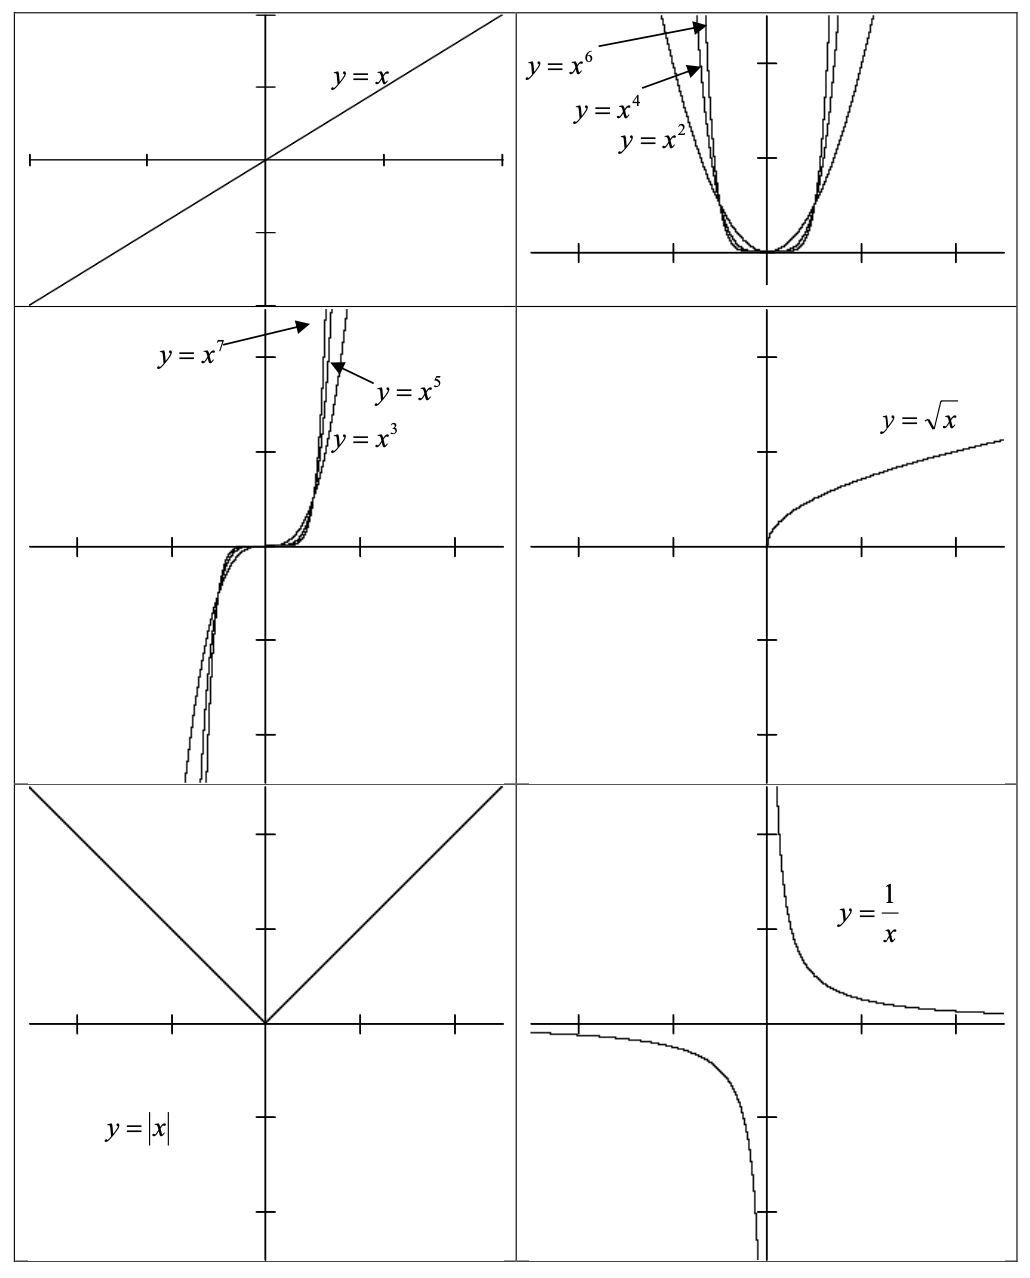
\includegraphics[width=0.7\linewidth]{chapter1/function1}\\
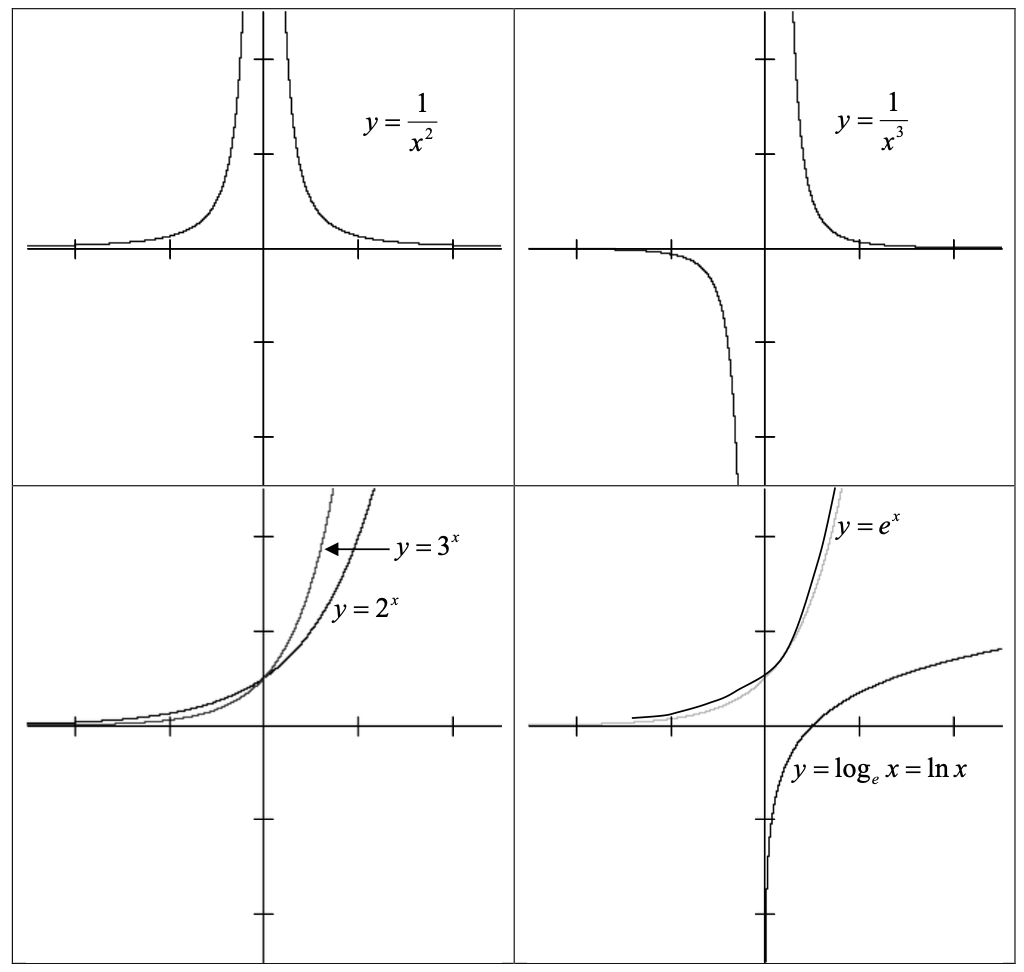
\includegraphics[width=0.7\linewidth]{chapter1/function2}


\makenewpage
% !TEX root = ../main.tex

\section{Limits}

\begin{myframe}[arc=10pt,auto outer arc]

\begin{enumerate}
\item One sided limits:
	\begin{enumerate}
		\item the limit of $f(x)$ as $x$ approaches $a$ from the right is $L$.
		\[
			\lim_{x\rightarrow a^+} f\left(x\right) = L
		\]
		\item the limit of $f(x)$ as $x$ approaches $a$ from the right is $L$.
		\[
			\lim_{x\rightarrow a^-} f\left(x\right) = L
		\]		
	\end{enumerate}
\item Two sided limits:

    \begin{enumerate}
    \item What is the limit of the following function as x approaches a?
    \[
    	\lim_{x\rightarrow a} f\left(x\right) = L \iff \lim_{x\rightarrow a^-} f\left(x\right) = \lim_{x\rightarrow a^+} f\left(x\right) = L
    \]
    
    \item If there is no sign in the limit notation, then you’re being asked for a two-sided limit. You only have a two-sided limit if your left and right limits agree. The existence of a limit from the left-hand side does not imply that you have a right-sided limit.
    When we say that something has a limit, then we mean that it has an actual numeric value.
    \end{enumerate}
    
\item Infinite limits
	\begin{enumerate}
		\item Increases without bound
		\[ \lim_{x \rightarrow a} f(x) = +\infty \]
		\item Decreases without bound
		\[ \lim_{x \rightarrow a} f(x) = -\infty \]
	\end{enumerate}

\item Limits at infinity
	\begin{enumerate}
	\item $\displaystyle \lim_{x \rightarrow +\infty} f(x) = L$: $\displaystyle f(x) \rightarrow L \textrm{ as } x \rightarrow +\infty$
	\item $\displaystyle \lim_{x \rightarrow -\infty} f(x) = L$: $\displaystyle f(x) \rightarrow L \textrm{ as } x \rightarrow -\infty$
	\end{enumerate}

\item Vertical asymptote

If $\displaystyle \left( \lim_{x\rightarrow a^-} f\left(x\right) = +\infty \textrm{ or } 
 \lim_{x\rightarrow a^-} f\left(x\right) = -\infty \right)$
and 
$\displaystyle \left( \lim_{x\rightarrow a^+} f\left(x\right) = +\infty  \textrm{ or }  
 \lim_{x\rightarrow a^+} f\left(x\right) = -\infty \right)$,
 
 then \textbf{the line $x=a$} is called the \textbf{vertical asymptote} of
 the graph of a function $f$.
 
 \item Horizontal asymptote
If  $\displaystyle \lim_{x\rightarrow +\infty} f\left(x\right) = L$ or $\displaystyle \lim_{x\rightarrow -\infty} f\left(x\right) = L$, then \textbf{the line $y=L$} is called the \textbf{horizontal asymptote} of the graph of a function f

\end{enumerate}

\end{myframe}

\newpage
\noindent Consider the graph of a function %f(x)$ below:

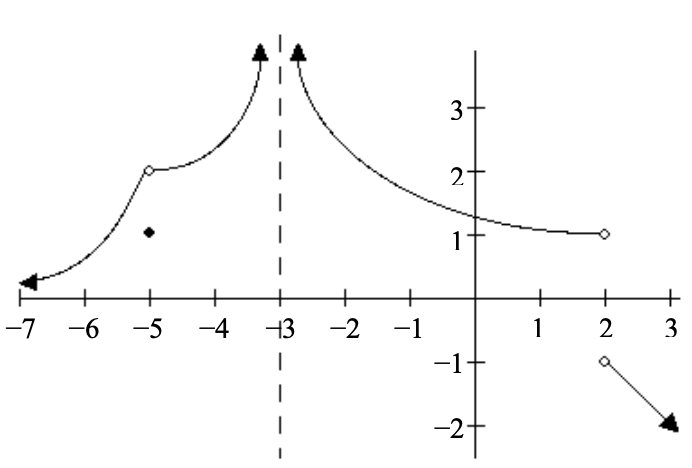
\includegraphics[width=0.7\linewidth]{chapter1/limits}

\noindent Find:

\pairofprobsans%
{$\displaystyle f(2)$}{undefined}
{$\displaystyle \lim_{x \rightarrow 2^-} f(x)$}{$\displaystyle 1$}

\pairofprobsans%
{$\displaystyle \lim_{x \rightarrow 2^+} f(x)$}{$\displaystyle -1$}
{$\displaystyle \lim_{x \rightarrow 2} f(x)$}{undefined}

\pairofprobsans%
{$\displaystyle f(-5)$}{$\displaystyle 1$}
{$\displaystyle \lim_{x \rightarrow -5^-} f(x)$}{$\displaystyle 2$}

\pairofprobsans%
{$\displaystyle \lim_{x \rightarrow -5^+} f(x)$}{$\displaystyle 2$}
{$\displaystyle \lim_{x \rightarrow -5} f(x)$}{$\displaystyle 2$}

\pairofprobsans%
{$\displaystyle f(-3)$}{undefined}
{$\displaystyle \lim_{x \rightarrow -3^-} f(x) $}{$\displaystyle +\infty$}

\pairofprobsans%
{$\displaystyle \lim_{x \rightarrow -3^+} f(x)$}{$\displaystyle +\infty$}
{$\displaystyle \lim_{x \rightarrow -3} f(x)$}{$\displaystyle +\infty$}

\pairofprobsans%
{$\displaystyle \lim_{x \rightarrow -\infty} f(x)$}{$\displaystyle 0$}
{$\displaystyle \lim_{x \rightarrow +\infty} f(x)$}{$\displaystyle -\infty$}

\problemans%
{The vertical asymptote}{$\displaystyle x=-3$}


\makenewpage
% !TEX root = ../main.tex
\section{Computing Limits}
Evaluate the following limits.

\pairofprobsans%
{$\displaystyle \lim_{x\rightarrow3} \left(x + 2\right)$}{$5$}
{$\displaystyle \lim_{x\rightarrow3} \left(x^2 + x + 2\right)$}{$14$}

\pairofprobsans%
{$\displaystyle \lim_{x\rightarrow3} \frac{x + 2}{4 - x}$}{$5$}
{$\displaystyle \lim_{x\rightarrow4} {\left(4 - x\right)}$}{$0$}

\pairofprobsans%
{$\displaystyle \lim_{x\rightarrow4} \frac{4 - x}{x - 2}$}{$0$}
{$\displaystyle \lim_{x\rightarrow4} \frac{x - 2}{4 - x}$}{does not exists}


%%%% GUIDES
\qrfigure{chapter1/qr/Computing-Limits.png}{Scan for guides}\makenewpage
% !TEX root = ../main.tex

\section{Computing Limits - Case $\displaystyle \lim_{x\rightarrow a} f(x)=\frac{0}{0}$}

Evaluate the following limits.

\problemans%
{$\displaystyle \lim_{x\rightarrow-3} {\frac{x^2 + 5x + 6}{x + 3} }$}{$-1$}

\problemans%
{$\displaystyle \lim_{x\rightarrow0} {\frac{x}{\sqrt{x + 4} - 2} }$}{$4$}

%%%% GUIDES
\qrfigure{chapter1/qr/Limits-of-Indeterminate-Form-of-Type-of-0divide0.png}{Scan for guides}\makenewpage
% !TEX root = ../main.tex

\section{Computing Limits at $\infty$}

\subsection{Odd vs Even Positive Integer Powers}

Evaluate the following limits.

\pairofprobsans
{$\displaystyle \lim_{x\rightarrow2} x$}{2}
{$\displaystyle \lim_{x\rightarrow+\infty} x$}{$+\infty$}

\pairofprobsans
{$\displaystyle  \lim_{x\rightarrow-2} x$}{$-2$}
{$\displaystyle \lim_{x\rightarrow-\infty} x$}{$-\infty$}

\pairofprobsans
{$\displaystyle  \lim_{x\rightarrow2} 3$}{$3$}
{$\displaystyle \lim_{x\rightarrow+\infty} 3$}{$3$}

\pairofprobsans
{$\displaystyle \lim_{x\rightarrow-2} x^3$}{$-8$}
{$\displaystyle \lim_{x\rightarrow-\infty} x^3$}{$-\infty$}

\pairofprobsans
{$\displaystyle \lim_{x\rightarrow-2} x^2$}{$+4$}
{$\displaystyle \lim_{x\rightarrow-\infty} x^2$}{$+\infty$}

\pairofprobsans
{$\displaystyle \lim_{x\rightarrow-2} (-x^2)$}{$-4$}
{$\displaystyle \lim_{x\rightarrow-\infty} (-x^2)$}{$-\infty$}

\pairofprobsans
{$\displaystyle \lim_{x\rightarrow-2} (-x^3)$}{$+8$}
{$\displaystyle \lim_{x\rightarrow-\infty} (-x^3)$}{$+\infty$}

\problemans
{$\displaystyle \lim_{x\rightarrow+\infty} (-3x)$}{$-\infty$}

%%%% GUIDES
\qrfigure{chapter1/qr/Limits-at-Infinity}{Scan for guides}

\makenewpage\subsection{Polynomials}

\begin{myframe}[arc=10pt,auto outer arc]
	Limits at $\infty$ for polynomials matches limits at $\infty$ of its highest degree term.
\end{myframe}

\noindent Evaluate the following limits.

\problemans%
{$\displaystyle \lim_{x\rightarrow+\infty} (3x^4 + 2x + 3)$}{$+\infty$}

\problemans%
{$\displaystyle \lim_{x\rightarrow+\infty} (-3x^4 + 2x + 3)$}{$-\infty$}

\problemans%
{$\displaystyle \lim_{x\rightarrow-\infty} (3x^4 + 2x + 3)$}{$+\infty$}

\problemans%
{$\displaystyle \lim_{x\rightarrow-\infty} (-3x^4 + 2x + 3)$}{$-\infty$}

\problemans%
{$\displaystyle \lim_{x\rightarrow-\infty} (2x^3 + 2x + 3)$}{$-\infty$}

\problemans%
{$\displaystyle \lim_{x\rightarrow-\infty} (-2x^3 + 2x + 3)$}{$+\infty$}

%%%% GUIDES
\qrfigure{chapter1/qr/Limits-at-Infinity-Polynomials}{Scan for guides}

\makenewpage\subsection{Rational Functions}
\begin{myframe}[arc=10pt,auto outer arc]
	\begin{enumerate}
		\item Divide the numerator and denominator by the highest power $x$ that occurs in the denominator.
		\item $\displaystyle \lim_{x\rightarrow+\infty} \frac{1}{x} = \lim_{x\rightarrow-\infty} \frac{1}{x} = 0$
	\end{enumerate}
\end{myframe}

\noindent Evaluate the following limits.

\problemans%
{$\displaystyle \lim_{x\rightarrow+\infty} \frac{2x + 4}{5x - 3}$}{$\frac{2}{5}$}

\problemans%
{$\displaystyle \lim_{x\rightarrow-\infty} \frac{2x^2 + 4}{5x - 3}$}{$-\infty$}

%%%% GUIDES
\qrfigure{chapter1/qr/Limits-at-Infinity-Rational}{Scan for guides}

\makenewpage\subsection{Radical Functions}
\begin{myframe}[arc=10pt,auto outer arc]
	\begin{enumerate}
		\item Find the limit first, and subsequently, calculate the square root..
		\item $\displaystyle \lim_{x\rightarrow+\infty} \frac{1}{x} = \lim_{x\rightarrow-\infty} \frac{1}{x} = 0$
	\end{enumerate}
\end{myframe}

\noindent Evaluate the following limits.

\problemans%
{$\displaystyle \lim_{x\rightarrow+\infty} \sqrt{\frac{2x + 4}{5x - 3}}$}{$\sqrt{\frac{2}{5}}$}

\problemans%
{$\displaystyle \lim_{x\rightarrow+\infty} \frac{\sqrt{x^2 + 1}}{2x - 3}$}{$\frac{1}{2}$}

\problemans%
{$\displaystyle \lim_{x\rightarrow-\infty} \frac{\sqrt{x^2 + 1}}{2x - 3}$}{$-\frac{1}{2}$}

%%%% GUIDES
\qrfigure{chapter1/qr/Limits-at-Infinity-Radicals}{Scan for guides}

\makenewpage\subsection{Indeterminate Form of Type $\infty - \infty$}

\noindent Evaluate the following limits.

\problemans%
{$\displaystyle \lim_{x\rightarrow+\infty} \left(\sqrt{x^2-3x} - x\right)$}{$-\frac{3}{2}$}

\problemans%
{$\displaystyle \lim_{x\rightarrow+\infty} \left(\sqrt{x^2+3} - x\right)$}{$0$}

%%%% GUIDES
\qrfigure{chapter1/qr/Limits-Indeterminate-Form-of-Type-Infinity-Infinity}{Scan for guides}
\makenewpage
% !TEX root = ../main.tex
\section{Limits of Trigonometric Functions}

%\subsection{Limits of Trigonometric Functions I}

\noindent Evaluate the following limits.

\problemans%
{$\displaystyle \lim_{x\rightarrow0} \left(\sin{\left(x\right)}\right)$}{$0$}

\problemans%
{$\displaystyle \lim_{x\rightarrow0} \left(\cos{\left(x + 1 \right)}\right)$}{$\cos{ \left( 1 \right) }$}

\problemans%
{$\displaystyle \lim_{x\rightarrow+\infty} \left(\cos{\left( \frac{1}{x} \right)}\right)$}{$1$}

%\makenewpage\subsection{Limits of Trigonometric Functions II}
\newpage

\begin{myframe}[arc=10pt,auto outer arc]
\begin{enumerate}
\item $\displaystyle \lim_{x\rightarrow 0} \frac{\sin{x}}{x} = \lim_{x\rightarrow 0} \frac{x}{\sin{x}} = 1$
\item $\displaystyle \lim_{x\rightarrow 0} \frac{\cos{x} - 1}{x} = \lim_{x\rightarrow 0} \frac{x}{1- \cos{x}} = 0$
\end{enumerate}
\end{myframe}

\noindent Evaluate the following limits.

\problemans%
{$\displaystyle \lim_{x\rightarrow 0} \left( \frac{\sin{\left( 3x \right)}}{x} \right)$}{$3$}

\problemans%
{$\displaystyle \lim_{x\rightarrow 0} \left( \frac{\sin{\left( 3x \right)} - x\cos{(3x)}}{x} \right)$}{$2$}

%\makenewpage\subsection{Limits of Trigonometric Functions III}
\newpage

%\begin{myframe}[arc=10pt,auto outer arc]
%\begin{enumerate}
%	\item $\displaystyle \lim_{x\rightarrow 0} \frac{\sin{x}}{x} = \lim_{x\rightarrow 0} \frac{x}{\sin{x}} = 1$
%	\item $\displaystyle \lim_{x\rightarrow 0} \frac{\cos{x} - 1}{x} = \lim_{x\rightarrow 0} \frac{x}{1- \cos{x}} = 1$
%\end{enumerate}
%\end{myframe}

\noindent Evaluate the following limits.

\problemans%
{$\displaystyle \lim_{x\rightarrow \frac{\pi}{2}} \frac{\pi + x\cos{(x)}}{2x - \sin{(x)}}$}{$\frac{\pi}{\pi-1}$}

\problemans%
{$\displaystyle \lim_{x\rightarrow 0}  \frac{\sin{(5x})}{\sin{(4x)}}$}{$\frac{5}{4}$}

\problemans%
{$\displaystyle \lim_{x\rightarrow 0}  \frac{x}{\tan{(3x)}}$}{$\frac{1}{3}$}

\problemans%
{$\displaystyle  \lim_{h\rightarrow 0} \frac{f(x+h) - f(x)}{h}$ if $\displaystyle f(x) = \cos{(x)}$}{$-\sin{(x)}$}

%%%% GUIDES
\qrfigure{chapter1/qr/Limits-of-Trigonometric-Functions}{Scan for guides}\makenewpage
% !TEX root = ../main.tex
\section{Continuity}

\begin{myframe}[arc=10pt,auto outer arc]
$f$ is continuous at $x=a$ if:
\begin{enumerate}
	\item $f\left(a\right)$ is defined.
	\item $\displaystyle \lim_{x\rightarrow a} f\left(x\right) \textrm{exists} \Leftrightarrow \lim_{x\rightarrow a^+} f\left(x\right) = \lim_{x\rightarrow a^-} f\left(x\right)$.
	\item $\displaystyle \lim_{x\rightarrow a} f\left(x\right) = f\left(a\right) = L$.
\end{enumerate}
\end{myframe}

\problemans{Determine whether the function $\displaystyle f\left(x\right)=\frac{4x+12}{x^2-9}$ is continuous at $x=0$.}{continuous}

\problemans{Determine whether the function $\displaystyle f\left(x\right)=\frac{4x+1}{x^2-9}$ is continuous at $x=-3$.}{discontinuous}


\newpage
\problemans{Determine whether the following function is continuous at $x=3$. \\
	$ f\left(x\right) =
	\begin{cases} 
		2x^2 - 5 & x< 3 \\
		4x + 1 & x\geq 3 
	\end{cases}$}{continuous}

\problemans{Find the value(s) of $k$ if $f$ is continuous at $x=1$. \\ $ f\left(x\right) =
	\begin{cases} 
		x^2 - 2 & x < 1 \\
		kx - 4 & x \geq 1 
	\end{cases}$}{3}

%%%% GUIDES
\qrfigure{chapter1/qr/Continuity.png}{Scan for guides}
\makenewpage

%Chapter 2
\chapter{Differentiation}
% !TEX root = ../main.tex
\section{Definition of Derivative}

\begin{myframe}[arc=10pt,auto outer arc]
	\centering $\displaystyle f'(x) = \lim_{h\rightarrow0} \frac{f(x+h) - f(x)}{h}$
\end{myframe}

\noindent Find the derivative of $f$ using the definition of derivative.

\problemans%
{$\displaystyle f(x) = x + 4$}{$1$}

\problemans%
{$\displaystyle f(x) = x^2 + 4$}{$2x$}

\newpage
\problemans%
{$\displaystyle f(x) = \sqrt{x + 4}$}{$\frac{1}{2\sqrt{x+4}}$}

\problemans%
{$\displaystyle f(x) = \frac{1}{x + 4}$}{$-\frac{1}{(x+4)^2}$}

\newpage
\problemans%
{$\displaystyle f(x) =\sin{(x)}$}{$\cos{(x)}$}

\problemans%
{$\displaystyle f(x) =\cos{(x)}$}{$-\sin{(x)}$}

%%%% GUIDES
\qrfigure{chapter2/qr/Definition-of-Derivative}{Scan for guides}\makenewpage
% !TeX root = ../main.tex
\section{Techniques of Differentiation}

\begin{myframe}[arc=10pt,auto outer arc]
	\begin{enumerate}
		\item Power Rule: $\left( x^n \right)' = nx^{n-1};  n\in\Re$
		\item Product Rule: $\left[u\left(x\right)v\left(x\right)\right]' = v(x) u'(x) + u(x) v'(x)$
		\item Quotient Rule: $\displaystyle\left[\frac{u\left(x\right)}{v\left(x\right)}\right]' = \frac{v(x) u'(x) - u(x) v'(x) }{ v(x)^2}$
	\end{enumerate}
\end{myframe}

\noindent Find the derivative $f'\left(x\right)$.

\pairofprobsans%
{$\displaystyle f\left(x\right) = 3x^8 - 2x^5 + 6x + 1$}{$24x^7 - 10x^4 + 6$}%
{$\displaystyle f\left(x\right) = \left(4x^2 - 1\right)\left(7x^3 + x\right)$}{$140x^4 - 9x^2 - 1$}

\pairofprobsans%
{$\displaystyle f\left(x\right) = \frac{x^2 - 1}{x^4 + 1}$}{$\displaystyle \frac{-2x^5 + 4x^3 + 2x}{(x^4+1)^2}$}%
{$\displaystyle f\left(x\right) = x^2 \tan{x}$}{$\displaystyle (\tan{x})(2x) + x^2 \sec^2{x}$}

\newpage
\begin{myframe}[arc=10pt,auto outer arc]
	\begin{enumerate}
		\item Derivative of logarithmic function: $\displaystyle \left[\log_b(u(x))\right]' = \frac{u'(x)}{u(x) \ln{b}}$
		\item Derivative of natural logarithmic function: $\displaystyle \left[\ln(u(x))\right]' = \frac{u'(x)}{u(x)}$
		\item Derivative of exponential function: $\displaystyle \left[b^{u(x)}\right]' = b^{u(x)} (\ln{b} )u'(x)$
		\item Derivative of exponential function: $\displaystyle \left[e^{u(x)}\right]' = b^{u(x)} u'(x)$
	\end{enumerate}
\end{myframe}

\pairofprobsans%
{$\displaystyle f\left(x\right) = \log_2{(x^2+1})$}{$\displaystyle \frac{2x}{(x^2+ 1) \ln{2}}$}%
{$\displaystyle f\left(x\right) = \ln{(x^2 + 1)}$}{$\displaystyle \frac{2x}{x^2+ 1}$}

\pairofprobsans%
{$\displaystyle f\left(x\right) = 2^{\sin{(x)}}$}{$2^{\sin{x}}(\cos{(x)})\ln{2}$}%
{$\displaystyle f\left(x\right) = e^{\cos{x}}$}{$\displaystyle -e^{\cos{x}}\sin{x}$}\makenewpage
% !TEX root = ../main.tex
\section{The Chain Rule}


\begin{myframe}[arc=10pt,auto outer arc]
	\centering Chain Rule: $\displaystyle (f\circ g)'(x) = f'(g(x)) \times g'(x)$
\end{myframe}

\pairofprobsans%
{$\displaystyle f\left(x\right) = (x^3 + 2x - 3)^4$}{$\displaystyle 4(x^3 + 2x - 3)^{3}(3x^2 + 2)$}%
{$\displaystyle f\left(x\right) = 4{\sin{(x^3)}}$}{$\displaystyle 12x^2 \cos{(x^3)}$}

\problemans%
{$\displaystyle f\left(x\right) = \frac{1}{x^3 + 2x - 3}$}{$\displaystyle -\frac{3x^2 + 2}{(x^3 + 2x - 3)^2}$}%

%%%% GUIDES
\qrfigure{chapter2/qr/Chain-Rule}{Scan for guides}\makenewpage
% !TEX root = ../main.tex
\section{Implicit Differentiation}

\pairofprobsans%
{$\displaystyle \frac{d}{dx}\left(x^2 + 3x + 4\right)$}{$\displaystyle 2x + 3$}%
{$\displaystyle \frac{d}{dx}\left[\left(x^2 + 3x + 4\right)^5\right]$}{$\displaystyle 5\left(x^2 + 3x + 4\right)^4 \left(2x + 3\right)$}

\pairofprobsans%
{Find $\displaystyle \frac{dy}{dx}$ for $y = f(x)$.}{$\displaystyle \frac{df}{dx}$}%
{Find $\displaystyle \frac{dy}{dx}$ for $y = [f(x)]^5$.}{$\displaystyle 5[f(x)]^4\frac{df}{dx}$}

\newpage
\pairofprobsans%
{Find $\displaystyle \frac{dy}{dx}$ for $y^3 = [f(x)]^5$.}{$\displaystyle \frac{5[f(x)]^4\frac{df}{dx}}{3y^2}$}%
{Find $\displaystyle \frac{dy}{dx}$ for $y^3 = \left(x^2 + 3x + 4\right)^5$.}{$\displaystyle \frac{5\left(x^2 + 3x + 4\right)^4 \left(2x+3\right)}{3y^2}$}

\pairofprobsans%
{Find $\displaystyle \frac{dy}{dx}$ for $5y^2 + \sin{y}= x^2$.}{$\displaystyle \frac{2x}{10y + \cos{y}}$}%
{Find $\displaystyle \frac{dy}{dx}$ for $x^3 + y^3 = 3xy$ (Folium of Descartes).}{$\displaystyle \frac{y - x^2}{y^2 - x}$}

%%%% GUIDES
\qrfigure{chapter2/qr/Implicit-Differentiation}{Scan for guides}\makenewpage
% !TEX root = ../main.tex
\section{Equation of Tangent Line}

\begin{myframe}[arc=10pt,auto outer arc]
	\centering $\displaystyle y - y_1 = m\left( x - x_1 \right)$
\end{myframe}

\problemans{Find the equation of tangent line to $f\left(x\right)=x^2 + 1$ at $x=2$.}{$y = 4x - 3$}

\problemans{Find the equation of tangent line to $f\left(x\right) = 2x^2$ at the point $\left(3, 18\right)$.}{$y = 12x - 18$}

%%%% GUIDES
\qrfigure{chapter2/qr/Equation-of-Tangent-Line}{Scan for guides}\makenewpage
% !TEX root = ../main.tex
\section{Linear Approximations and Differentials}

\begin{myframe}[arc=10pt,auto outer arc]
\begin{enumerate}
\item Local Linear Approximation of $f$ at $x_0$
\[ f(x) \approx f(x_0) + f'(x_0) (x - x_0) \]
\item Differentials: For the function y = f (x), we define the following:
\begin{enumerate}
\item $dx$, called the differential of $x$, given by the relation $dx = \delta x$
\item $dy$, called the differential of $y$, given by the relation $dy = f'(x)dx$
\end{enumerate}
\end{enumerate}
\end{myframe}

\problemans{Find the local linear approximation of $\displaystyle f\left(x\right)=\sqrt{x}$ at $x_0=4$.}{$\displaystyle \frac{x + 4}{4}$}

\newpage
\problemans{Use differentials to approximate $\displaystyle \sqrt{3.98}$.}{$\displaystyle 1\frac{199}{200}$}

\problemans{Use differentials to approximate $\displaystyle \sqrt{4.02} - \frac{1}{\sqrt{4.02}}$.}{$\displaystyle 1 \frac{81}{160}$}

%%%% GUIDES
\qrfigure{chapter2/qr/Local-Linear-Approximations-and-Differentials}{Scan for guides}

\makenewpage

%Chapter 3
\chapter{Applications of Differentiation}
% !TEX root = ../main.tex
\section{Related Rates}

\begin{myframe}[arc=10pt,auto outer arc]
	Find the rate at which some quantity is changing by relating the quantity to other quantities whose rates of change is known.
	
	\begin{enumerate}
	    \item Given $y = f(x)$ and $x = g(t)$ \\and a constant rate of change $\displaystyle \frac{dx}{dt}$.
		\item Find the changes of $y$ in time (or rate of change or how fast is the changing) when $x=`something'$.
		\item $\displaystyle \frac{dy}{dt} = \left. \frac{df}{dx} \right\vert_{x=`something'} \times \frac{dx}{dt}$.
	\end{enumerate}
\end{myframe}


\problemans{The value of $x$ is increasing at a constant rate of 4. How fast is $y = 3x^2 + 2$ changing at the instant $x=2$.}{$\displaystyle \frac{dy}{dt} = 48$}

\problemans{The value of $y$ is decreasing at a constant rate of 1. $x^2 + y^2 = 625$. How fast is $x$ changing at the instant $x=7$.}{$\displaystyle \frac{dx}{dt} = \frac{24}{7}$}

%%%% GUIDES
\qrfigure{chapter3/qr/Related-Rates}{Scan for guides}\makenewpage
% !TeX root = ../main.tex
\section{Critical Points}

\begin{myframe}[arc=10pt,auto outer arc]
	$x=c$ is a critical point of $f(x)$ if:
	\begin{enumerate}
		\item $f'(c) = 0$, or
		\item $f'(c)$ does not exists
	\end{enumerate}
\end{myframe}

\noindent Determine all the critical point(s) for the following functions:

\problemans{$\displaystyle x^2 - 4x + 3$}{$\displaystyle x=2$}

\problemans{$\displaystyle x^3 - 3x + 2$}{$\displaystyle x = \{-1, 1\}$}

\problemans{$\displaystyle \frac{x-1}{x+2}$}{$\displaystyle x=-2$}

%%%% GUIDES
\qrfigure{chapter3/qr/Critical-Points}{Scan for guides}

%---------------------------------------------------------------
\makenewpage
\section{Intervals of Increasing and Decreasing Functions}

\begin{myframe}[arc=10pt,auto outer arc]
	Let $f$ be a function that is continuous on a closed interval $[a, b]$ and is differentiable on the open interval $(a, b)$.
	
	\begin{center}
		\begin{tabular}{ | c | c | c | c |}
			\hline
			 & \multicolumn{3}{| c |}{$x$ on interval $(a, b)$} \\ 
			 \hline
			$f'(x)$ & $+$ & $-$ & $0$ \\ 
			\hline 
			$f(x)$ & increasing, $f \uparrow$  & decreasing $\downarrow$  & constant \\
			\hline
		\end{tabular}
	\end{center}
\end{myframe}


\noindent Determine the intervals where the following functions are decreasing or decreasing.

\problemans{$\displaystyle x^2 - 4x + 3$}{decreasing: $\{(-\infty, 2)\}$; increasing: $\{(2, +\infty)\}$}

\problemans{$\displaystyle x^3 - 3x + 2$}{decreasing: $\{(-1, 1)\}$; increasing: $\{(-\infty, -1), (1, +\infty)\}$}

\problemans{$\displaystyle \frac{x-1}{x+2}$}{decreasing: none; increasing: $\{(-\infty, -2), (-2, +\infty)\}$}

%%%% GUIDES
\qrfigure{chapter3/qr/Increasing-and-Decreasing-Functions}{Scan for guides}

%---------------------------------------------------------------
\makenewpage
\section{Concavity and Inflection Points}

\begin{myframe}[arc=10pt,auto outer arc]
	Let $f$ be twice differentiable on the open interval $(a, b)$.
	
	\begin{center}
		\begin{tabular}{ | c | c | c |}
			\hline
			& \multicolumn{2}{| c |}{$x$ on interval $(a, b)$} \\ 
			\hline
			$f''(x)$ & $+$ & $-$ \\ 
			\hline 
			$f(x)$ & concave up, $f \cup$  & concave down $\cap$ \\
			\hline
		\end{tabular}
	\end{center}
	
	$x=c$ is an \textbf{inflection point} of $f(x)$ if the concavity changes at $x=c$.
\end{myframe}

\noindent 

\problemans{$\displaystyle x^2 - 4x + 3$}{concave up: $\{(-\infty, +\infty)\}$; concave down: none; no inflection point}

\problemans{$\displaystyle x^3 - 3x + 2$}{concave up: $\{(0, +\infty)\}$; concave down: $\{(-\infty, 0)\}$; inflection point: $x=0$}

\problemans{$\displaystyle \frac{x-1}{x+2}$}{concave up: $\{(-\infty, -3)\}$; concave down: $\{(-2, +\infty)\}$; no inflection point}

%%%% GUIDES
\qrfigure{chapter3/qr/Concavity-and-Inflection-Points}{Scan for guides}

%---------------------------------------------------------------



\makenewpage
% !TEX root = ../main.tex
\section{Asymptotes}

\begin{myframe}[arc=10pt,auto outer arc]
\begin{enumerate}
	\item \textbf{vertical asymptotes:} vertical lines which correspond to the zeroes of the denominator of rational function.
	\item \textbf{horizontal asymptotes:} $\displaystyle \lim_{x\rightarrow \pm \infty} f(x)$
\end{enumerate}
\end{myframe}

\problemans{$\displaystyle f(x) = \frac{x-1}{x+2}$}{vertical asymptotes: $x=-2$; horizontal asymptotes: $y=1$}

%%%% GUIDES
\qrfigure{chapter3/qr/Vertical-and-Horizontal-Asymptotes}{Scan for guides}

%--------------------------------------
\makenewpage
\section{Curve Sketching: Even Polynomial Function}

\begin{myframe}[arc=10pt,auto outer arc]
	Steps:
	\begin{enumerate}
\item $y-\textrm{intercepts}$
\item $x-\textrm{intercepts}$
\item Intervals of decrease and increase
\item Concavity and inflection points
\item Relative extrema
\item Sketch graph
	\end{enumerate}
\end{myframe}

\noindent Sketch the graph of the following function.

\problem{$\displaystyle f(x) = x^2 - 4x + 3$}{}

%%%% GUIDES
\qrfigure{chapter3/qr/Sketch-Even-Polynomial-Graphs}{Scan for guides}

%--------------------------------------
\makenewpage
\section{Curve Sketching: Odd Polynomial Function}

\begin{myframe}[arc=10pt,auto outer arc]
	Steps:
	\begin{enumerate}
		\item $y-\textrm{intercepts}$
		\item $x-\textrm{intercepts}$
		\item Intervals of decrease and increase
		\item Concavity and inflection points
		\item Relative extrema
		\item Sketch graph
	\end{enumerate}
\end{myframe}

\noindent Sketch the graph of the following function.

\problem{$\displaystyle f(x) = x^3 - 3x + 2$}{}

%%%% GUIDES
\qrfigure{chapter3/qr/Sketch-Odd-Polynomial-Graphs}{Scan for guides}

%--------------------------------------
\makenewpage
\section{Curve Sketching: Rational Function}

\begin{myframe}[arc=10pt,auto outer arc]
	Steps:
	\begin{enumerate}
		\item $y-\textrm{intercepts}$
		\item $x-\textrm{intercepts}$
		\item Intervals of decrease and increase
		\item Concavity and inflection points
		\item Relative extrema
		\item \textbf{Asymptotes}
		\item Sketch graph
	\end{enumerate}
\end{myframe}

\noindent Sketch the graph of the following function.

\problem{$\displaystyle f(x) =\frac{x-1}{x+2}$}{}

%%%% GUIDES
\qrfigure{chapter3/qr/Sketch-Rational-Graphs}{Scan for guides}

%--------------------------------------\makenewpage  
% !TEX root = ../main.tex
\section{Rolle’s Theorem; Mean-Value Theorem}

\begin{myframe}[arc=10pt,auto outer arc]
\textbf{Mean Value Theorem:} $f$ is differentiable on $(a, b)$ and continuous on $[a, b]$. Then, there is at least one number $c$ in $(a, b)$ such that
		
		\[ f'(c) = \frac{f(b) - f(a)}{b - a} \]

\end{myframe}

\problemans{Determine all the numbers $c$ which satisfy the conclusions of the Mean Value Theorem for $f(x) = x^3 + 1$ on $(0, 2)$.}{$\displaystyle x = +1.1547$}


%--------------------------------------

\begin{myframe}[arc=10pt,auto outer arc]
\textbf{Rolle’s Theorems:} $f$ is differentiable on $(a, b)$.
		\[ f(a) = f(b) = 0\]
		
		Then, there is at least one number $c$ in $(a, b)$ such that 
		
		\[ f'(c) = 0\]

\end{myframe}

\problemans{Determine all the numbers $c$ which satisfy the conclusions of the Rolle's Theorem for $f(x) = x^3 - x$ on $[0, 1]$.}{$\displaystyle x =+0.5774$}

%%%% GUIDES
\qrfigure{chapter3/qr/Rolles-Theorem-Mean-Value-Theorem}{Scan for guides}\makenewpage
% !TEX root = ../main.tex
\section{Maximum and Minimum Values of a Function}
	
\begin{figure}[h!]
	\centering
	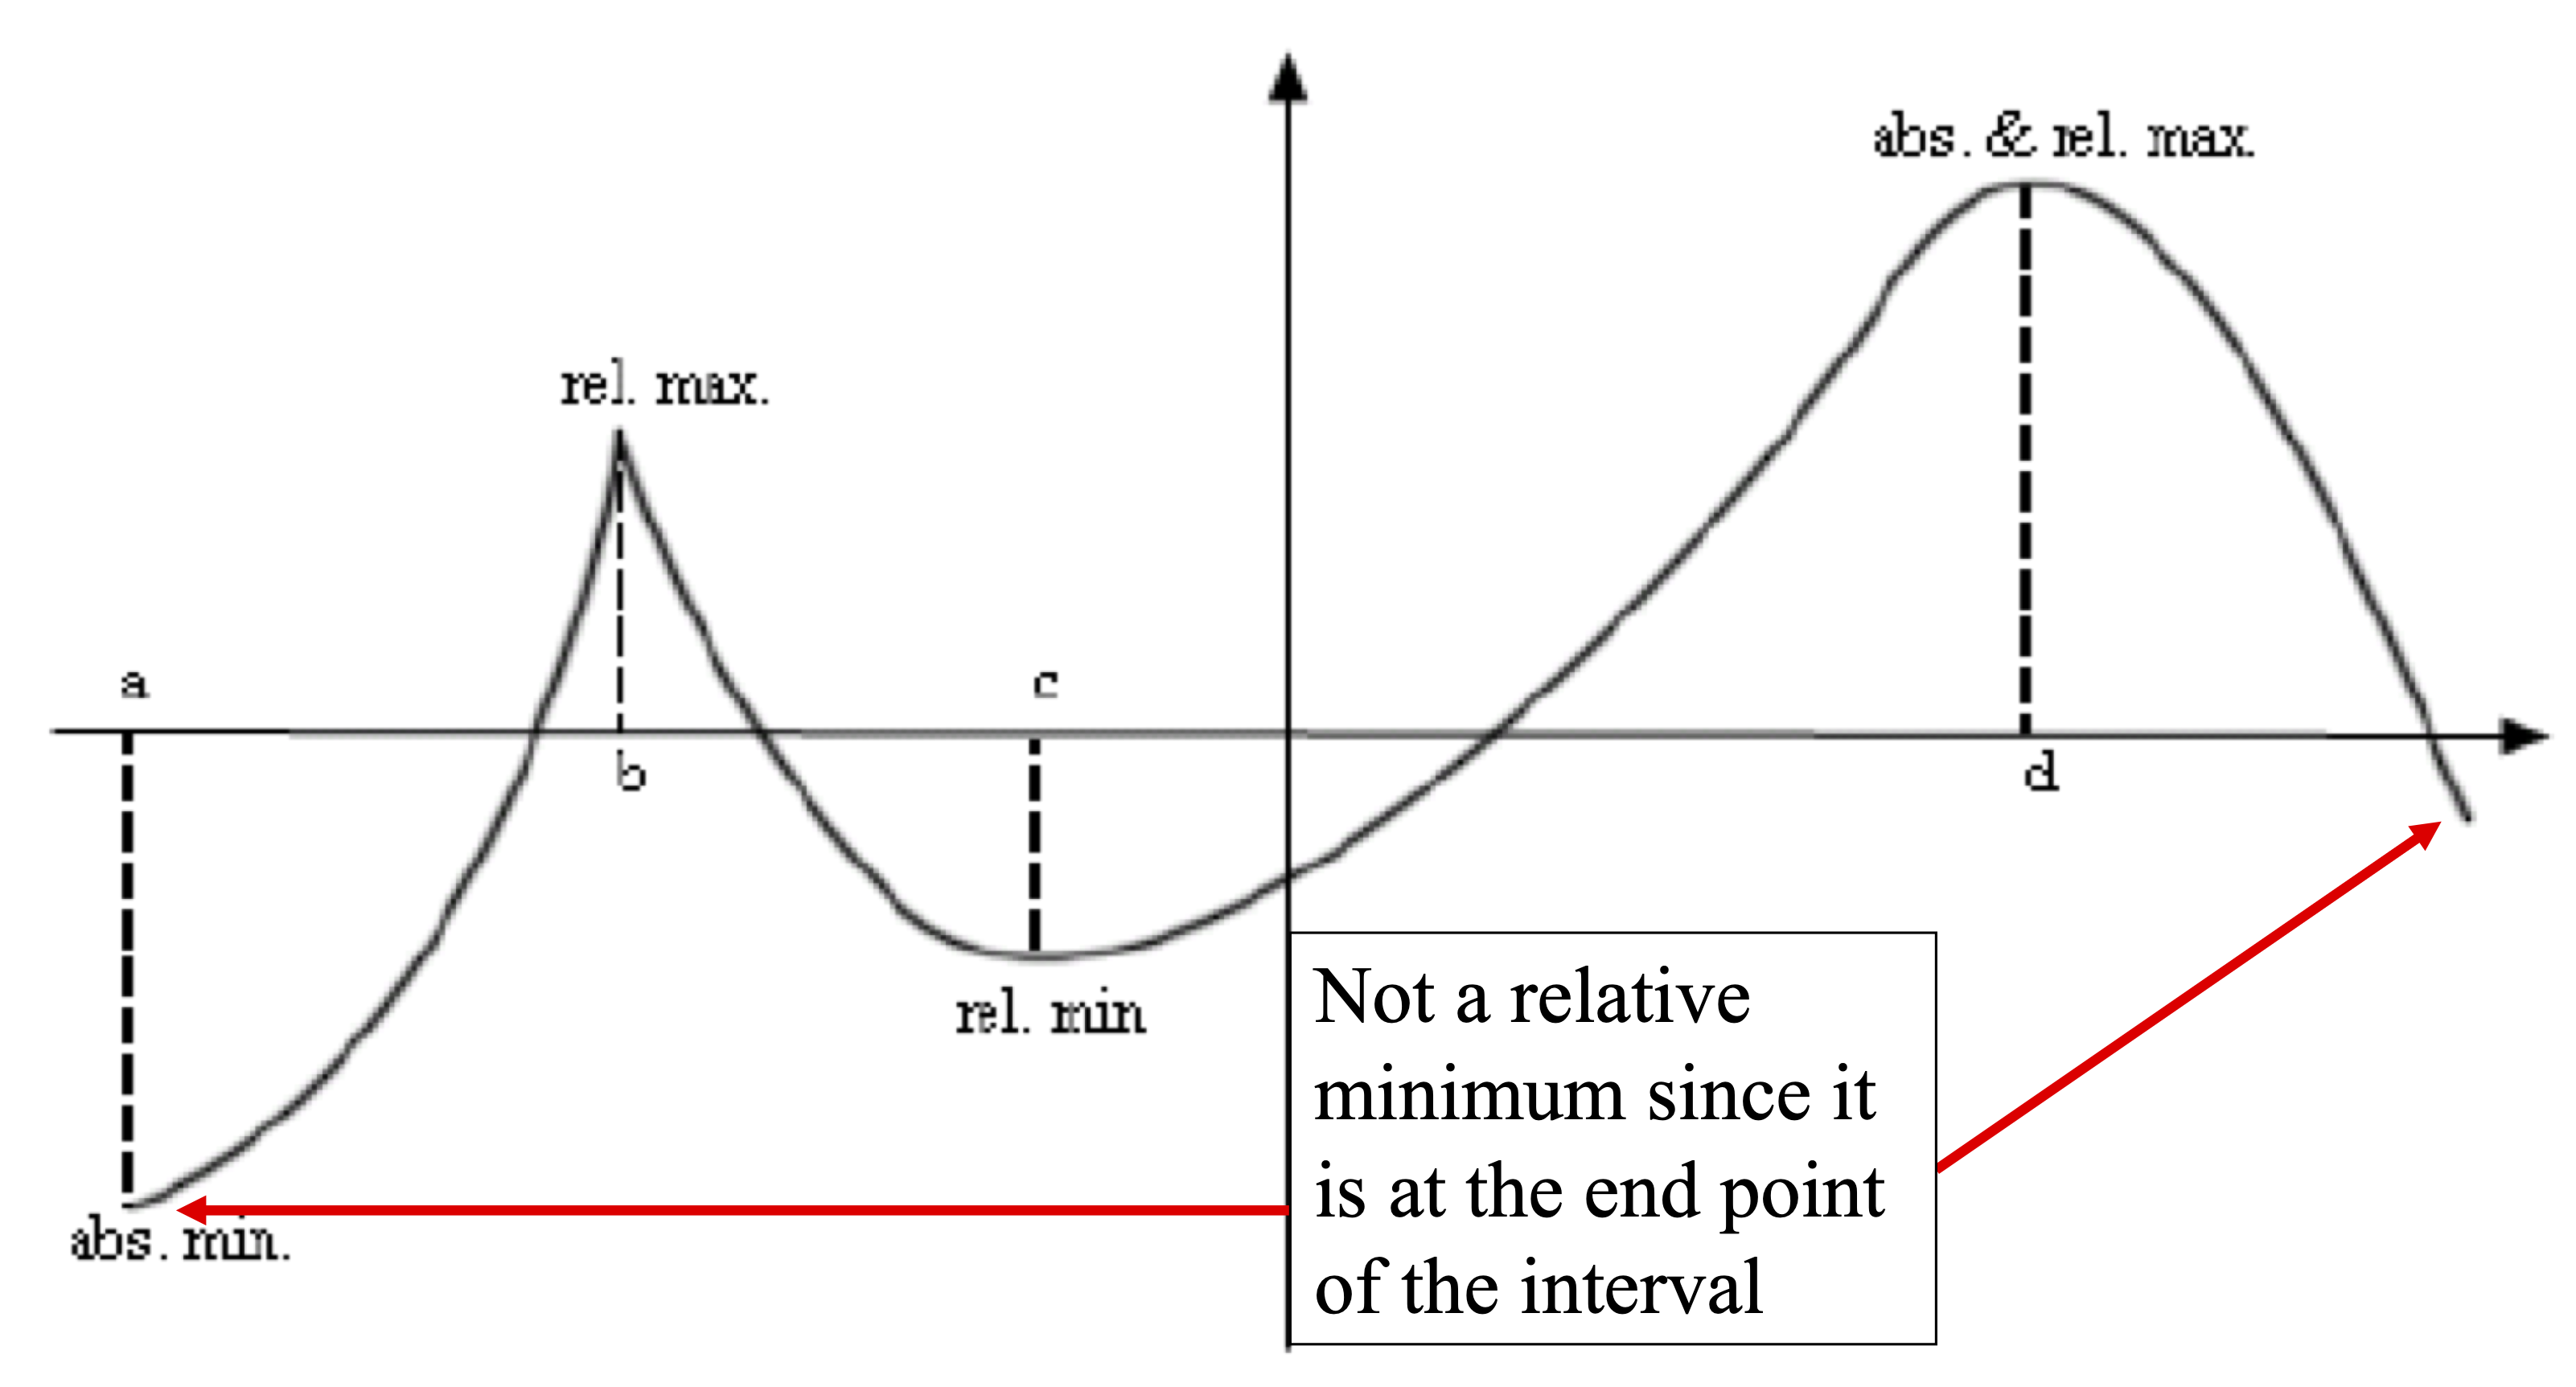
\includegraphics[width=0.9\linewidth]{chapter3/max-min}
	\caption{Maximum and minimum values.}
	\label{fig:max-min}
\end{figure}


\begin{myframe}[arc=10pt,auto outer arc]
	\begin{enumerate}
	\item \textbf{First Derivative test:} Suppose that $f$ is continuous at a critical number $x_0$.
	\begin{enumerate}
		\item  \textbf{Relative maximum} at $x_0$: $f'(x < x_0) > 0$ and $f'(x > x_0) < 0$
		\item  \textbf{Relative minimum} at $x_0$: $f'(x < x_0) < 0$ and $f'(x > x_0) > 0$
		\item  \textbf{No relative extremum} at $x_0$: No changes in sign of $f'(x_0)$
	\end{enumerate}
	
	
	\item \textbf{Second Derivative test:} Suppose that $f$ is twice differentiable $x_0$ and $f'(x_0)=0$.
		\begin{enumerate}
			\item \textbf{Relative minimum} at $x_0$: $f'' > 0$
			\item \textbf{Relative maximum} at $x_0$: $f'' < 0$
			\item \textbf{Inconclusive:} $f'' = 0$
    	\end{enumerate}
	
	\end{enumerate}
\end{myframe}

\newpage
\problem{Find the relative and absolute extremum values for $f(x)=2x^3-15x^2+36x$ on the interval $[1, 5]$.}

%%%% GUIDES
\qrfigure{chapter3/qr/Maximum-and-Minimum-Values}{Scan for guides}

\makenewpage

%Chapter 4
\chapter{Integration}
% !TEX root = ../main.tex

\section{The Indefinite Integral}

\begin{myframe}[arc=10pt,auto outer arc]
\[ \int b \,dx = bx + C
\]
\end{myframe}

\pairofprobsans%
{$\displaystyle \int 4 \,dx$}{$4x + C$}%
{$\displaystyle \int 0.4 \,dy$}{$0.4y + C$}%

\pairofprobsans%
{$\displaystyle \int \frac{1}{3} \,dx$}{$\displaystyle \frac{x}{3} + C$}%
{$\displaystyle \int e \,d\theta$}{$\displaystyle e \theta +C$}%

\pairofprobsans%
{$\displaystyle \int \sqrt{2} \,dx$}{$\displaystyle \sqrt{2}x + C$}%
{$\displaystyle \int (3 + \sqrt{2}) \,dz$}{$\displaystyle (3 + \sqrt{2})z + C$}%

\problemans%
{$\displaystyle \int \pi \,dx$}{$\pi x +C$}%

%-----------------------------
\newpage
\begin{myframe}[arc=10pt,auto outer arc]
	\[ \int x^r \,dx = \frac{x^{r+1}}{r + 1} + c; r\ne -1
	\]
\end{myframe}

\pairofprobsans%
{$\displaystyle \int x \,dx$}{$\displaystyle \frac{x^2}{2} + C$}%
{$\displaystyle \int 4x \,dx$}{$2x^2 + c$}%

\pairofprobsans%
{$\displaystyle \int x^2 \,dx$}{$\displaystyle \frac{x^3}{3} + C$}%
{$\displaystyle \int 3x^2 \,dx$}{$x^3 + c$}%

\pairofprobsans%
{$\displaystyle \int x^3 \,dx$}{$\displaystyle \frac{x^4}{4} + C$}%
{$\displaystyle \int 0.5x^3 \,dx$}{$\displaystyle \frac{x^4}{8} + C$}%

\problemans%
{$\displaystyle \int x^{0.5} \,dx$}{$\displaystyle \frac{x^{1.5}}{1.5} + C$}%

%-----------------------------

\newpage
\begin{myframe}[arc=10pt,auto outer arc]
	\[ \int x^r \,dx = \frac{x^{r+1}}{r + 1} + c; r\ne -1
	\]
\end{myframe}

\problemans%
{$\displaystyle \int (x + x^2) \,dx$}{$\displaystyle \frac{x^2}{2} + \frac{x^3}{3} + C$}%

\problemans%
{$\displaystyle \int (3x^6 - 2x^2 + 7x + 1) \,dx$}{$\displaystyle 3\frac{x^7}{7} - 2\frac{x^3}{3} + 7\frac{x^2}{2} + x + C$}%

%-----------------------------

\newpage
\begin{myframe}[arc=10pt,auto outer arc]
	\[ \int x^r \,dx = \frac{x^{r+1}}{r + 1} + c; r\ne -1
	\]
\end{myframe}

\pairofprobsans
{$\displaystyle \int \sqrt{x} \,dx$}{$\displaystyle \frac{2}{3}x^{\frac{3}{2}}+ C$}%
{$\displaystyle \int \sqrt[3]{x} \,dx$}{$\displaystyle \frac{3}{4} x^{\frac{4}{3}} + C$}%

\problemans%
{$\displaystyle \int \sqrt{x^3} \,dx$}{$\displaystyle \frac{2}{5} x^{\frac{5}{2}} + C$}%

%-----------------------------


\newpage
\begin{myframe}[arc=10pt,auto outer arc]
	\[ \int x^r \,dx = \frac{x^{r+1}}{r + 1} + c; r\ne -1
	\]
\end{myframe}

\pairofprobsans%
{$\displaystyle \int (x+2)(x-3) \,dx$}{$\displaystyle \frac{x^3}{3} - \frac{x^2}{2} -6x + C$}%
{$\displaystyle \int \frac{x^3 + 2x^2}{x} \,dx$}{$\displaystyle \frac{x^3}{3} + x^2 + C$}%

\pairofprobsans%
{$\displaystyle \int \frac{1}{x^3}  \,dx$}{$\displaystyle -\frac{1}{2x^2} + C$}%
{$\displaystyle \int \frac{3}{x^2} \,dx$}{$\displaystyle -\frac{3}{x} + C$}%

%-----------------------------


\newpage
\begin{myframe}[arc=10pt,auto outer arc]
	\begin{enumerate}
	\item $\displaystyle \int x^r \,dx = \frac{x^{r+1}}{r + 1} + c; r\ne -1$
	\item $\displaystyle \int \frac{1}{u} \, du = \ln{u} + C$
	\item $\displaystyle \int e^u \, du = e^u + C$
	\item $\displaystyle \int b^u \, du = \frac{b^u}{\ln{b}} + C$
	\end{enumerate}
\end{myframe}

\pairofprobsans%
{$\displaystyle \int \frac{2}{x} \,dx$}{$\displaystyle 2\ln{x} + C$}%
{$\displaystyle \int 5e^x \,dx$}{$\displaystyle 5e^x + C$}%

\pairofprobsans%
{$\displaystyle \int 2^x \,dx$}{$\displaystyle \frac{2^x}{\ln{2}} + C$}%
{$\displaystyle \int \pi^x \,dx$}{$\displaystyle \frac{\pi^x}{\ln{\pi}} + C$}%

%-----------------------------


\newpage
\begin{myframe}[arc=10pt,auto outer arc]
	\begin{enumerate}
		\item $\displaystyle \int \sin{(x)} \,dx = -\cos{(x)} + C$
		\item $\displaystyle \int \cos{(x)} \,dx = \sin{(x)} + C$
		\item $\displaystyle \int \sec^2{(x)} \,dx = \tan{(x)} + C$
		\item $\displaystyle \int \csc^2{(x)} \,dx = -\cot{(x)} + C$
		\item $\displaystyle \int \sec{(x)} \tan{(x)} \,dx = \sec{(x)} + C$
		\item $\displaystyle \int \csc{(x)} \cot{(x)} \,dx = -\csc{(x)} + C$
	\end{enumerate}
\end{myframe}


\pairofprobsans%
{$\displaystyle \int 2\sin{(x)} \,dx$}{$\displaystyle -2\cos{(x)} + C$}%
{$\displaystyle \int 10\cos{(x)} \,dx$}{$\displaystyle 10\sin{(x)} + C$}%

\pairofprobsans%
{$\displaystyle \int 5\sec^2{(x)} \,dx$}{$\displaystyle 5\tan{(x)} + C$}%
{$\displaystyle \int 2\csc^2{(x)} \,dx$}{$\displaystyle -2\cot{(x)} + C$}%


\pairofprobsans%
{$\displaystyle \int 10 \sec{(x)} \tan{(x)} \,dx$}{$\displaystyle 10\sec{(x)} + C$}%
{$\displaystyle \int 2\csc{(x)} \cot{(x)} \,dx$}{$\displaystyle -2\csc{(x)} + C$}%
%-----------------------------

%%%% GUIDES
\qrfigure{chapter4/qr/The-Indefinite-Integrals}{Scan for guides}
\makenewpage
%!TEX root = ../main.tex

\section{Integration by Substitution}

\noindent Evaluate the following integral:

\pairofprobsans%
{$\displaystyle \int (x^2 + 1)^{50} 2x \,dx$}{$\displaystyle \frac{(x^2 + 1)^{51}}{51} + C$}%
{$\displaystyle \int (x^2 + 1)^{50} x \,dx$}{$\displaystyle \frac{(x^2 + 1)^{51}}{102} + C$}%

\pairofprobsans%
{$\displaystyle \int \left(x - 8\right)^5\,dx$}{$\displaystyle \frac{\left(x-8\right)^6}{6} + C$}%
{$\displaystyle \int \frac{1}{\left(\frac{x}{3} - 8\right)^5}\,dx$}{$\displaystyle -\frac{3}{4(\frac{x}{3} -8)^4} + C$}%

\pairofprobsans%
{$\displaystyle \int \sin{(x+9)} \,dx$}{$\displaystyle -\cos{(x + 9)} + C$}%
{$\displaystyle \int \cos{(5x)} \,dx$}{$\displaystyle \frac{\sin{(5x)}}{5} + C$}%

\newpage
\pairofprobsans%
{$\displaystyle \int \left( \frac{1}{x^2} +\sec^2(\pi x) \right) \,dx$}{$\displaystyle -\frac{1}{x} + \frac{\tan{(\pi x)}}{\pi}+ C$}%
{$\displaystyle \int \sin^2{(x)} \cos{(x)}  \,dx$}{$\displaystyle \frac{\sin^3{(x)}}{3} + C$}%

\pairofprobsans%
{$\displaystyle \int \frac{\cos{(\sqrt{x})}}{\sqrt{x}} \,dx$}{$\displaystyle 2\sin{\left(\sqrt{x}\right)} + C$}%
{$\displaystyle \int t^4 \sqrt[3]{3 - 5t^5}  \,dt$}{$\displaystyle -\frac{3}{100} \left(3-5t^5 \right)^\frac{4}{3} + C$}%

\newpage
\pairofprobsans%
{$\displaystyle \int x^2\sqrt{x-1} \,dx$}{$\displaystyle \frac{2}{7}(x-1)^\frac{7}{2} + \frac{4}{5}(x+1)^\frac{5}{2} + \frac{2}{3}(x-1)^\frac{3}{2} + C$}%
{$\displaystyle \int \frac{3x^2}{\left( x^3 - 1 \right)^5} \,dx$}{$\displaystyle -\frac{\left( x^3 - 1 \right)^{-4}}{4} + C$}%

\problemans%
{$\displaystyle \int \cos^3{(x)}  \,dx$}{$\displaystyle \sin{(x)} - \frac{\sin^3{(x)}}{3} + C$}%

%%%% GUIDES
\qrfigure{chapter4/qr/Integration-by-Substitution}{Scan for guides}
\makenewpage
% !TEX root = ../main.tex
\section{The Definite Integral}

\begin{myframe}[arc=10pt,auto outer arc]
\begin{enumerate}
\item \textbf{First Fundamental Theorem of Calculus:} If $f$ is continuous on $[a, b]$ and $F$ is antiderivative of $f$ on $[a, b]$, then
\[
\int_a^b f(x) \,dx = F(b) - F(a)
\]

\item \textbf{Area} $=$ \\
The sum of the areas \textbf{above the $x$-axis} and \textbf{under} the graph
$-$ \\
The sum of the areas \textbf{under the $x$-axis} and \textbf{above} the graph \\
$\displaystyle = A_2 - A_1 - A_3$ \\
$\displaystyle = \int_0^5 f(x) \,dx$ 

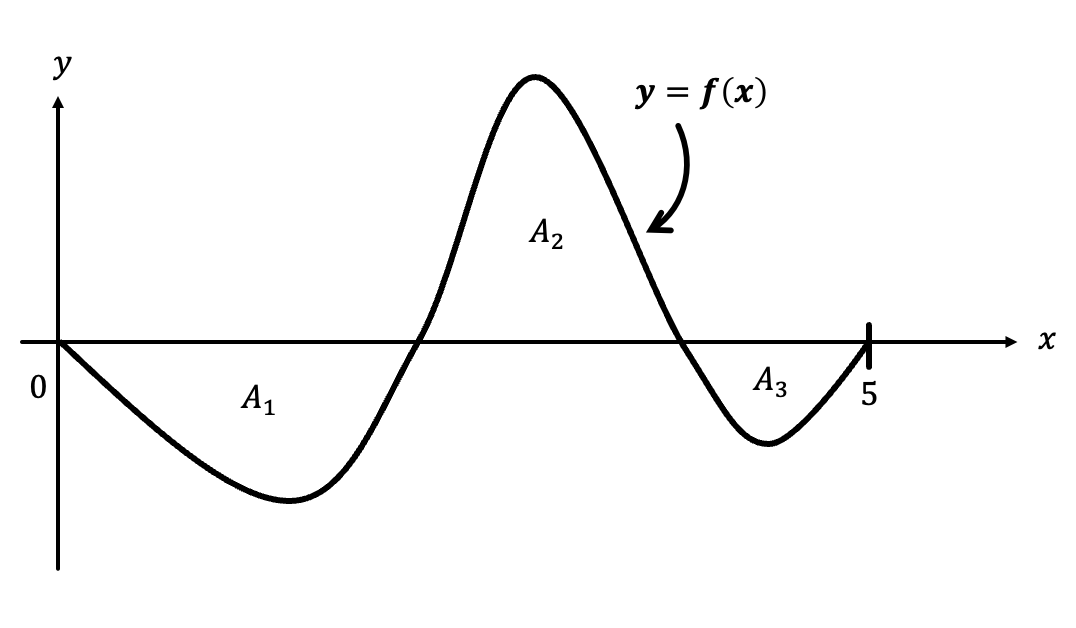
\includegraphics[width=0.7\linewidth]{chapter4/area}

\end{enumerate}
\end{myframe}

\pairofprobsans%
{$\displaystyle \int_{-1}^4 \frac{1}{x^2} \, dx$ }{undefined}
{$\displaystyle \int_{1}^2 x \, dx $ }{$\displaystyle \frac{3}{2}$}

\newpage
\pairofprobsans%
{$\displaystyle \int_0^3 \left( 9-x^2 \right) \, dx$ }{$\displaystyle 18$}
{$\displaystyle \int_0^{\frac{\pi}{3}} \sec^2{(x)} \, dx $ }{$\displaystyle \sqrt{3}$}

\pairofprobsans%
{$\displaystyle \int_1^1 x^2 \, dx$ }{$\displaystyle 0$}
{$\displaystyle \int_4^0 x \, dx $ }{$\displaystyle -8$}

\newpage
\problemans%
{Evaluate the integral $\displaystyle \int_0^6 f(x) dx$ if
	$ \displaystyle f(x) = \begin{cases} 
		x^2 & x < 2 \\
		3x-2 & x\geq 2 
	\end{cases}
	$.
	}%
{$\displaystyle \frac{128}{3}$}

%%%% GUIDES
\qrfigure{chapter4/qr/Definite-Integral}{Scan for guides}
%----------------------


\makenewpage
% !TEX root = ../main.tex
\section{Evaluating Definite Integrals by Substitution}

\pairofprobsans%
{$\displaystyle \int_0^2 x\left( x^2+1 \right)^3 \,dx $}%
{$78$}%
{$\displaystyle \int_0^{\frac{\pi}{8}} \sin^5{(2x)} \cos{(2x)} \,dx$}%
{$\displaystyle \frac{1}{96}$}%

\problemans{$\displaystyle \int_2^5 (2x-5)(x-3)^9 \,dx $}{$\displaystyle \frac{52233}{110}$}

%%%% GUIDES
\qrfigure{chapter4/qr/Evaluating-Definite-Integrals-by-Substitution}{Scan for guides}
\makenewpage
% !TEX root = ../main.tex
\section{The Second Fundamental Theorem of Calculus}
 
\begin{myframe}[arc=10pt,auto outer arc]
If $f$ is continuous on interval $I$, $A$ is any number in $I$, $F$ is an antiderivative of $F$ on $I$.
	\begin{enumerate}
\item $\displaystyle F(x) = \int_a^x f(t) \,dt \implies F'(x) = \frac{d}{dx} \int_a^x f(t) \,dt = f(x) $
\item $\displaystyle F(x) = \int_a^{g(x)} f(t) \,dt \implies F'(x) = \frac{d}{dx} \int_a^{g(x)} f(t) \,dt = f(g(x)) g'(x) $
\end{enumerate}
\end{myframe}

\pairofprobsans%
{$\displaystyle \frac{d}{dx} \int_1^x t^3 \,dt $}{$\displaystyle x^3$}%
{$\displaystyle \frac{d}{dx} \int_1^x \frac{\sin{(t)}}{t} \,dt $}{$\displaystyle \frac{\sin{(x)}}{x}$}%

\problemans%
{$\displaystyle \frac{d}{dx} \int_2^{3x^2} 4u \,du $}{$\displaystyle 72x^3$}%

%%%% GUIDES
\qrfigure{chapter4/qr/The-Second-Fundamental-Theorem-of-Calculus}{Scan for guides}

\makenewpage
% !TEX root = ../main.tex

\section{Mean-Value Theorem for Integrals}

\begin{myframe}[arc=10pt,auto outer arc]
If $f$ is continuous on $[a, b]$, then there is at least one number $c$
in $[a, b]$ such that

\[
\int_a^b f(x) \, dx = f(c)(b-a)
\]
\end{myframe}

\problemans%
{Find the value of $c$ in $[1, 4]$, if $f(x)=x^2$ that satisfy the Mean-Value theorem for integrals.}%
{$\displaystyle c=+\sqrt{7}$}%

%%%% GUIDES
\qrfigure{chapter4/qr/The-Mean-Value-Theorem-for-Integrals}{Scan for guides}\makenewpage

%Chapter 5
\chapter{Applications of Integration}
% !TEX root = ../main.tex

\section{Area Between Two Curves}

\begin{myframe}[arc=10pt,auto outer arc]
Area between two curves $y=f(x)$ (upper function) and $y=g(x)$ (lower function) on the interval $[a, b]$ is given by
\[
A = \int_a^b \left(f(x) - g(x)\right) \, dx
\]
\end{myframe}

\problemans%
{Find the area of the region\\
bounded above by $y = x + 6$,\\
bounded below by $y=x^2$, and \\
bounded of the sides by the lines $x=0$ and $x=2$.}
{$\frac{34}{3}$}%

\problemans%
{Find the area of the region\\
that is enclosed between the curves\\
$y=x^2$ and $y=x+6$.}%
{$\displaystyle \frac{125}{6}$}%

\newpage

\problemans%
{Find the area of the region\\
that is enclosed between the curves\\
$x=y^2$ and $y=x-2$.
}%
{$\displaystyle \frac{9}{2}$}%

\makenewpage
\begin{myframe}[arc=10pt,auto outer arc]
Area between two curves $x=f(y)$ (right function) and $x=g(y)$ (left function) on the interval $[c, d]$ is given by
\[
A = \int_a^b \left(f(x) - g(x)\right) \, dx
\]
\end{myframe}

\problemans%
{Find the area of the region\\
that is enclosed between the curves\\
$x=y^2$ and $y=x-2$.
}%
{$\frac{9}{2}$}%

%\problemans%
%{Find the area of the region\\
%that is enclosed between the curves\\
%$x=y^2$ and $y=x-2$.
%}%
%{$\frac{9}{2}$}%

\makenewpage

\begin{myframe}[arc=10pt,auto outer arc]
	\noindent Area between a curve and the $x$-axis.
	
	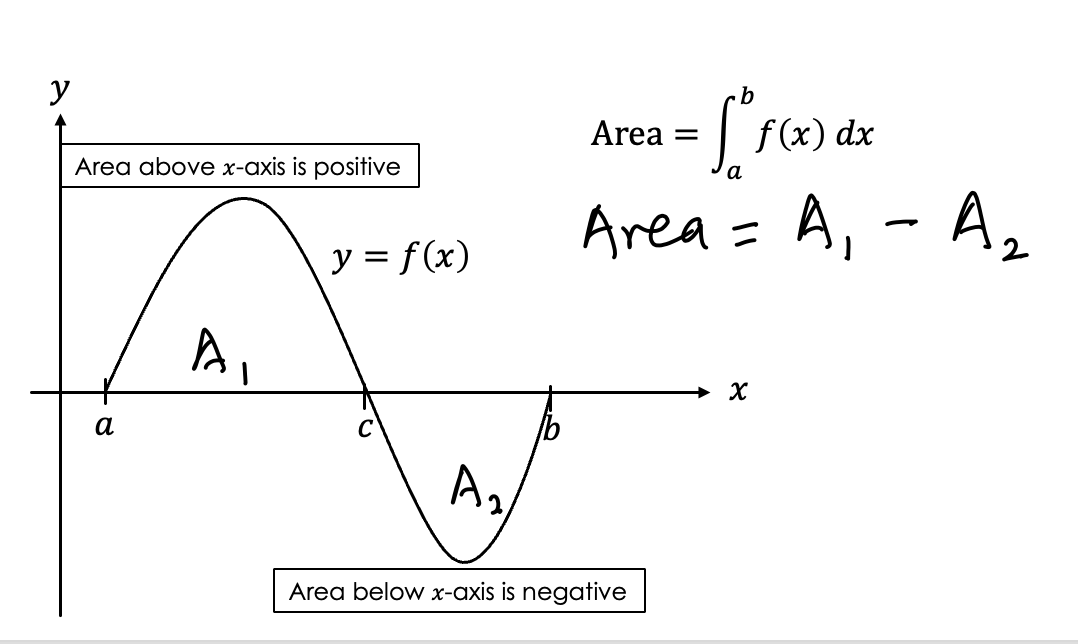
\includegraphics[width=0.7\linewidth]{chapter5/area}
\end{myframe}


\noindent Find the area under the curve $y=\cos{(x)}$ over the following intervals:

\pairofprobsans%
{$\displaystyle \left[0, \frac{\pi}{2}\right]$}{$1$}%
{$\displaystyle \left[\frac{\pi}{2}, \pi \right]$}{1}%

\problemans%
{$\displaystyle \left[0, \pi\right]$}{$$2}%

%%%% GUIDES
\qrfigure{chapter5/qr/Area-Between-Two-Curves}{Scan for guides}





\makenewpage
% !TEX root = ../main.tex

\section{Method of Disks/Washers (Perpendicular to the $x$-axis)}

\begin{myframe}[arc=10pt,auto outer arc]
		\centering
		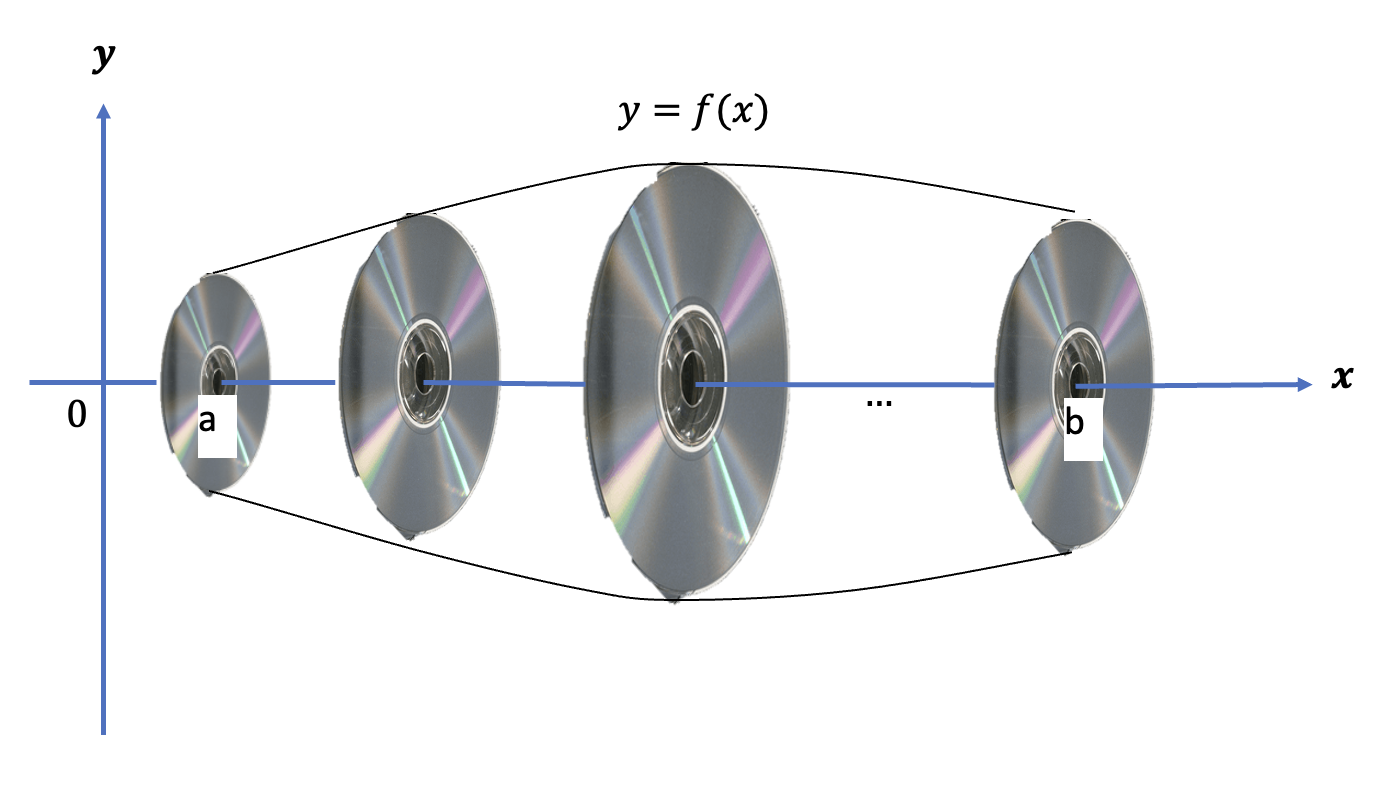
\includegraphics[width=0.7\linewidth]{chapter5/disc}
		
		\begin{enumerate}
			\item $\displaystyle \textrm{Area} = \pi\left(f(x) - 0\right)^2 = \pi\left(f(x) \right)^2$
			\item $\displaystyle \textrm{Volume} = \pi \int_{x=a}^b \left[ f(x) \right]^2 \, dx$
		\end{enumerate}
	
\end{myframe}

\problemans%
{Find the volume of the solid that is obtained when the region \\
	under the curve $y=\sqrt{x}$ over the interval $[1, 4]$  \\
	is revolved about the $x$-axis. 
}%
{$\displaystyle \frac{15}{2} \pi$}%

\newpage
\problemans%
{Find the volume of the solid that is obtained when the region \\
between the graph $\displaystyle f(x)=\frac{1}{2} + x^2$ and $g(x)=x$ over the interval $[0, 2]$ \\
is revolved about the $x$-axis.}%
{$\displaystyle \frac{69}{10}\pi$}%

\newpage
\problemans%
{Find the volume of the solid that is obtained when the region \\
	bounded by the graph $x=y^2$ and $y=x^2$ \\
	is revolved about the $x$-axis.
}%
{$\displaystyle \frac{3}{10} \pi$}%

\newpage
\problemans%
{Find the volume of the solid that is obtained when the region \\
	bounded by the graph $y=x^2$ and $y=x^3$ \\
	is revolved about the line $y=-1$. 
}%
{$\displaystyle \frac{47}{210}\pi$}%

%%%% GUIDES
\qrfigure{chapter5/qr/Method-of-Disks-Washers-Perpendicular-to-the-x-axis}{Scan for guides}

%-------------------------------------------------------
\makenewpage
\section{Method of Disks/Washers (Perpendicular to the $y$-axis)}

\begin{myframe}[arc=10pt,auto outer arc]
	\centering
	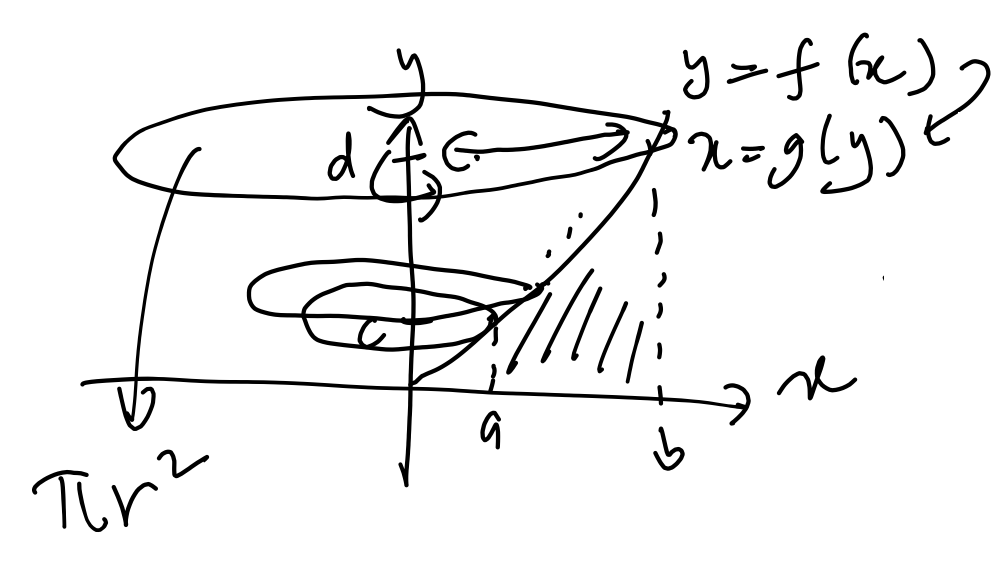
\includegraphics[width=0.7\linewidth]{chapter5/discy}
	
	\begin{enumerate}
		\item $\displaystyle \textrm{Area} = \pi\left(g(y) - 0\right)^2 = \pi \left[g(y)\right]^2$
		\item $\displaystyle \textrm{Volume} = \pi \int_{y=c}^d \left[ g(y) \right]^2 \, dy$
	\end{enumerate}
	
\end{myframe}

\problemans%
{Find the volume of the solid that is generated when the region \\
	enclosed by $y=\sqrt{x}$, $y=2$ and $x=0$ \\
	is revolved about the $y$-axis. 
}%
{$\displaystyle \frac{32}{5}\pi$}%

\newpage
\problemans%
{Find the volume of the solid that is generated when the region \\
	enclosed by $x=y^2$ and $y=x^2$ \\
	is revolved about the $y$-axis.   
}%
{$\displaystyle \frac{3}{10}\pi$}%

\newpage
\problemans%
{Find the volume of the solid that is generated when the region \\ 
	bounded by $y=x^2$ and $y=x^3$\\
	is revolved about the line $x=-1$.  
}%
{$\displaystyle \frac{4}{15}\pi$}%

%%%% GUIDES
\qrfigure{chapter5/qr/Method-of-Disks-Washers-Perpendicular-to-the-y-axis}{Scan for guides}





\makenewpage
% !TEX root = ../main.tex

\section{Cylindrical Shells (Revolved about the $y$-axis)
}

\begin{myframe}[arc=10pt,auto outer arc]
\centering
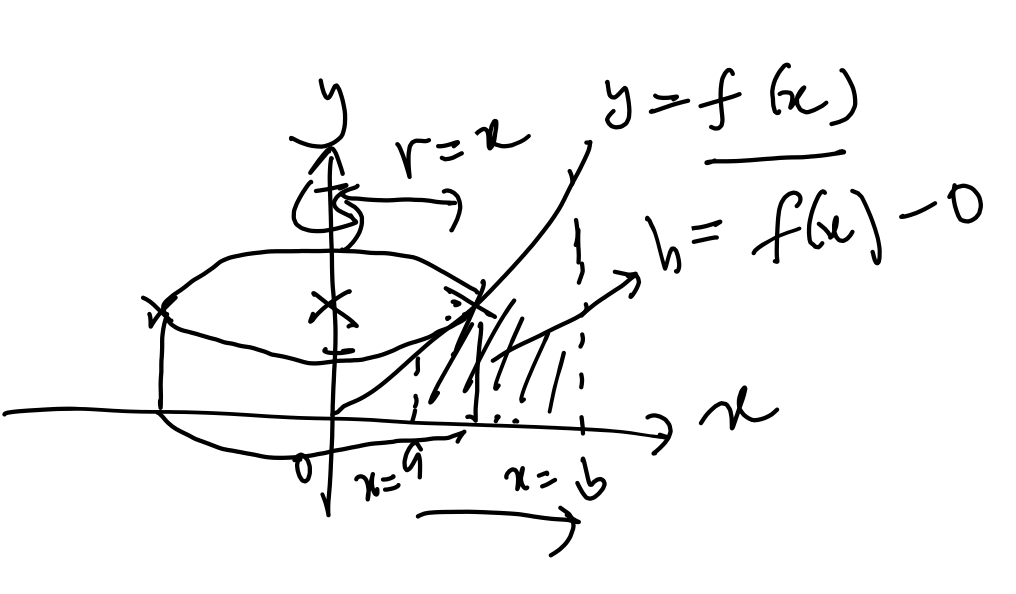
\includegraphics[width=0.7\linewidth]{chapter5/shelly}

\begin{enumerate}
	\item Volume of a cylinder, $V = 2\pi rh$
	\item $r = x$; $h = f(x)$
	\item  $\displaystyle V = 2\pi\int_{x=a}^b x f(x) \, dx$
\end{enumerate}

\end{myframe}

\problemans%
{Use cylindrical shells to find the volume of the solid generated \\
	when the region enclosed between $y=\sqrt{x}$, $x=1$, $x=4$ and the $x$-axis \\
	is revolved about the $y$-axis.
}%
{$\displaystyle \frac{124}{5} \pi$}%

\newpage
\problemans%
{Use cylindrical shells to find the volume of the solid generated \\
	when the region R in the first quadrant enclosed by $y=x$ and $y=x^2$  \\
	is revolved about the $y$-axis. 
}%
{$\displaystyle \frac{\pi}{6}$}%


\newpage
\problemans%
{Use cylindrical shells to find the volume of the solid generated \\
	when the region R in the first quadrant enclosed by $y=x$ and $y=x^2$ \\
	is revolved about the line $x=-1$. 
}%
{$\displaystyle \frac{\pi}{2}$}%

%%%% GUIDES
\qrfigure{chapter5/qr/Volumes-by-Cylindrical-Shells-revolved-about-the-y-axis}{Scan for guides}

%---------------------------
\makenewpage
\section{Cylindrical Shells (Revolved about the $x$-axis)}

\begin{myframe}[arc=10pt,auto outer arc]
\centering
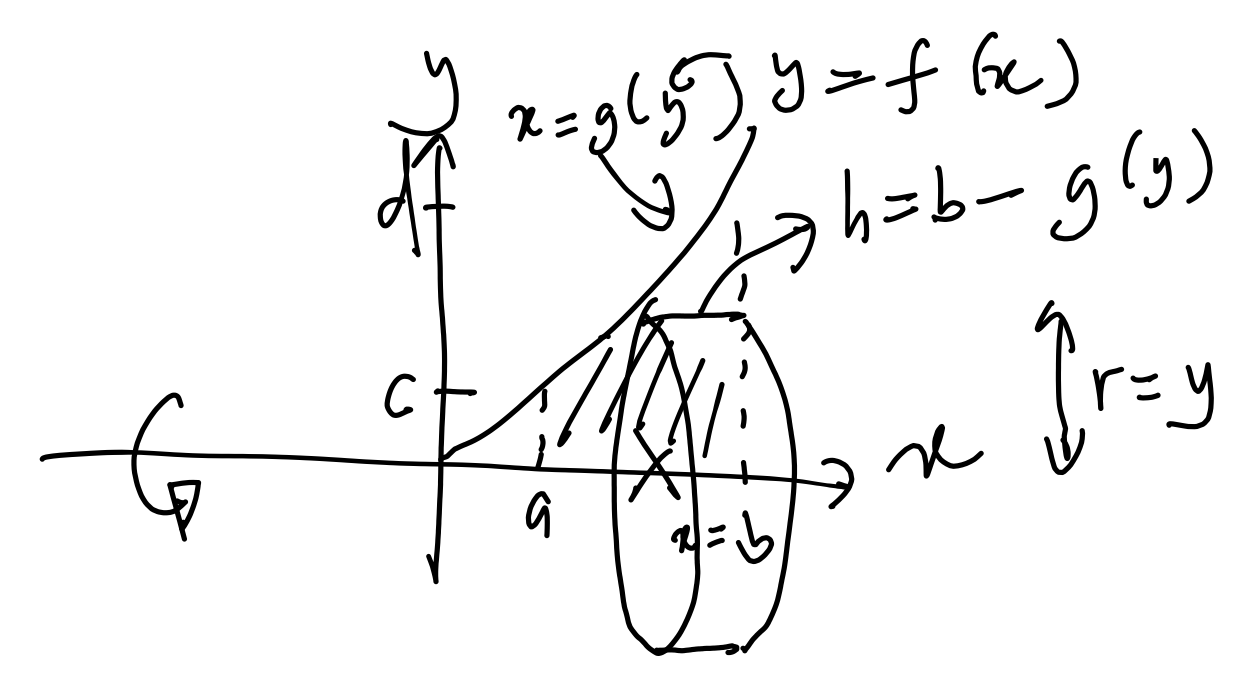
\includegraphics[width=0.7\linewidth]{chapter5/shellx}

\begin{enumerate}
	\item Volume of a cylinder, $V = 2\pi rh$
	\item $r = y$; $h = b - g(y)$
	\item  $\displaystyle V = 2\pi\int_{y=c}^d y \left(b - g(y)\right) \, dy$
\end{enumerate}

\end{myframe}

\problemans%
{Use cylindrical shells to find the volume of the solid generated \\
	when the region R under $y=x^2$ over the interval $[0, 2]$ \\ 
	is revolved about the $x$-axis.
}%
{$\displaystyle \frac{32}{5} \pi$}%


\newpage

\problemans%
{Use cylindrical shells to find the volume of the solid obtained \\
	by  rotating the region bounded by $x=\left(y-2\right)^2$ and $y=x$ \\ 
	about the  line $y=-1$.
}%
{$\displaystyle \frac{63}{2} \pi$}%

%%%% GUIDES
\qrfigure{chapter5/qr/Volumes-by-Cylindrical-Shells-revolved-about-the-x-axis}{Scan for guides}

\makenewpage
% !TEX root = ../main.tex

\section{Washer vs. Cylindrical Shell}

\noindent a) Find the volume of the solid generated \\
when the region enclosed between $y=\sqrt{x}$, $x=1$, $x=4$ and the $x$-axis \\
is revolved about the $y$-axis. 

\pairofprobsans%
{Washer}{$\displaystyle \frac{124}{5} \pi$}%
{Cylindrical Shell}{$\displaystyle \frac{124}{5} \pi$}%


\makenewpage
\noindent b) Find the volume of the solid generated \\
when the region $R$ in the first quadrant enclosed by $y=x$ and $y=x^2$ \\
is revolved about the $x$-axis. 

\pairofprobsans%
{Washer}{$\displaystyle \frac{2\pi}{15}$}%
{Cylindrical Shell}{$\displaystyle \frac{2\pi}{15}$}%

%\makenewpage
\noindent c) Find the volume of the solid generated \\
when the region $R$ in the first quadrant enclosed by $y=x$ and $y=x^2$ \\
is revolved about the $y$-axis. 

\pairofprobsans%
{Washer}{$\displaystyle \frac{\pi}{6}$}%
{Cylindrical Shell}{$\displaystyle \frac{\pi}{6}$}%

\makenewpage
\noindent d) Use cylindrical shells to find the volume of the solid generated \\
when the region R in the first quadrant enclosed by $y=x$ and $y=x^2$ \\
is revolved about the line $x=-1$. 

\pairofprobsans%
{Washer}{$\displaystyle \frac{\pi}{2}$}%
{Cylindrical Shell}{$\displaystyle \frac{\pi}{2}$}%

%%%% GUIDES
\qrfigure{chapter5/qr/Volumes-by-Disk-Washer-vs-Cylindrical-Shells}{Scan for guides}
\makenewpage

\backmatter
\appendix
%-------------
% To include past years or not
%-------------
\includepastyearstrue % Include past years
\includepastyearsfalse % does not include past years
\ifincludepastyears
  \input{past-years/past-years}
\fi
%\includepdf[pages={1},pagecommand={\section{Important Formulas I}}]{pdf/cheat/Formulas}
%\includepdf[pages={2},pagecommand={\section{Important Formulas II}}]{pdf/cheat/Formulas}

% !TEX root = ../main.tex
\chapter{Important Formulas}

\section{Derivatives and Integrals}

\begin{multicols}{2}
\noindent
\textbf{Derivatives:}
\begin{align*}
&\frac{d}{dx}c = 0 \\
&\frac{d}{dx}x^n = nx^{n-1} \\
&\frac{d}{dx}e^x = e^x \\
&\frac{d}{dx}a^x = \ln(a) \cdot a^x \\
&\frac{d}{dx}\ln(x) = \frac{1}{x} \\
&\frac{d}{dx}\log_a(x) = \frac{1}{x \ln(a)} \\
&\frac{d}{dx}\sin(x) = \cos(x) \\
&\frac{d}{dx}\cos(x) = -\sin(x) \\
&\frac{d}{dx}\tan(x) = \sec^2(x) \\
&\frac{d}{dx}\csc(x) = -\csc(x)\cot(x) \\
&\frac{d}{dx}\sec(x) = \sec(x)\tan(x) \\
&\frac{d}{dx}\cot(x) = -\csc^2(x) \\
&\frac{d}{dx}e^{u(x)} = u'(x)e^{u(x)} \\
&\frac{d}{dx}\ln|u(x)| = \frac{u'(x)}{u(x)}
\end{align*}

\columnbreak

\noindent
\textbf{Integrals:}
\begin{align*}
&\int 0\,dx = C \\
&\int x^n\,dx = \frac{x^{n+1}}{n+1} + C, \quad n \neq -1 \\
&\int e^x\,dx = e^x + C \\
&\int a^x\,dx = \frac{a^x}{\ln(a)} + C \\
&\int \frac{1}{x}\,dx = \ln|x| + C \\
&\int \frac{1}{x \ln(a)}\,dx = \log_a|x| + C \\
&\int \cos(x)\,dx = \sin(x) + C \\
&\int \sin(x)\,dx = -\cos(x) + C \\
&\int \sec^2(x)\,dx = \tan(x) + C \\
&\int \csc^2(x)\,dx = -\cot(x) + C \\
&\int \sec(x)\tan(x)\,dx = \sec(x) + C \\
&\int \csc(x)\cot(x)\,dx = -\csc(x) + C \\
&\int e^{u(x)}\,dx = \int e^{u(x)}u'(x)\,dx \quad \text{(use substitution)} \\
&\int \frac{1}{u(x)}u'(x)\,dx = \ln|u(x)| + C
\end{align*}
\end{multicols}

\newpage
\section{Trigonometric Identities, Index (Exponent) Rules and Logarithmic Properties}
\begin{multicols}{2}
\noindent

\noindent
\textbf{Index (Exponent) Rules:}
\begin{align*}
&a^m \cdot a^n = a^{m+n} \\
&a^m / a^n = a^{m-n} \\
&(a^m)^n = a^{mn} \\
&a^0 = 1 \quad (a \neq 0) \\
&a^{-n} = 1/a^n
\end{align*}

\noindent
\textbf{Logarithmic Properties:}
\begin{align*}
&\log_a(xy) = \log_a(x) + \log_a(y) \\
&\log_a\left(\frac{x}{y}\right) = \log_a(x) - \log_a(y) \\
&\log_a(x^n) = n\log_a(x) \\
&\log_a(a) = 1 \\
&\log_a(1) = 0
\end{align*}


\textbf{Trigonometric Identities:}
\begin{align*}
&\sin^2(x) + \cos^2(x) = 1 \\
&1 + \tan^2(x) = \sec^2(x) \\
&1 + \cot^2(x) = \csc^2(x) \\
&\sin(2x) = 2\sin(x)\cos(x) \\
&\cos(2x) = \cos^2(x) - \sin^2(x) \\
&\tan(2x) = \frac{2\tan(x)}{1 - \tan^2(x)}\\
&\sin(x + y) = \sin(x)\cos(y) + \cos(x)\sin(y) \\
&\sin(x - y) = \sin(x)\cos(y) - \cos(x)\sin(y) \\
&\cos(x + y) = \cos(x)\cos(y) - \sin(x)\sin(y) \\
&\cos(x - y) = \cos(x)\cos(y) + \sin(x)\sin(y) \\
&\tan(x + y) = \frac{\tan(x) + \tan(y)}{1 - \tan(x)\tan(y)} \\
&\tan(x - y) = \frac{\tan(x) - \tan(y)}{1 + \tan(x)\tan(y)}
\end{align*}

\end{multicols}

% !TEX root = ../main.tex
%\chapter{Cheat Sheets}
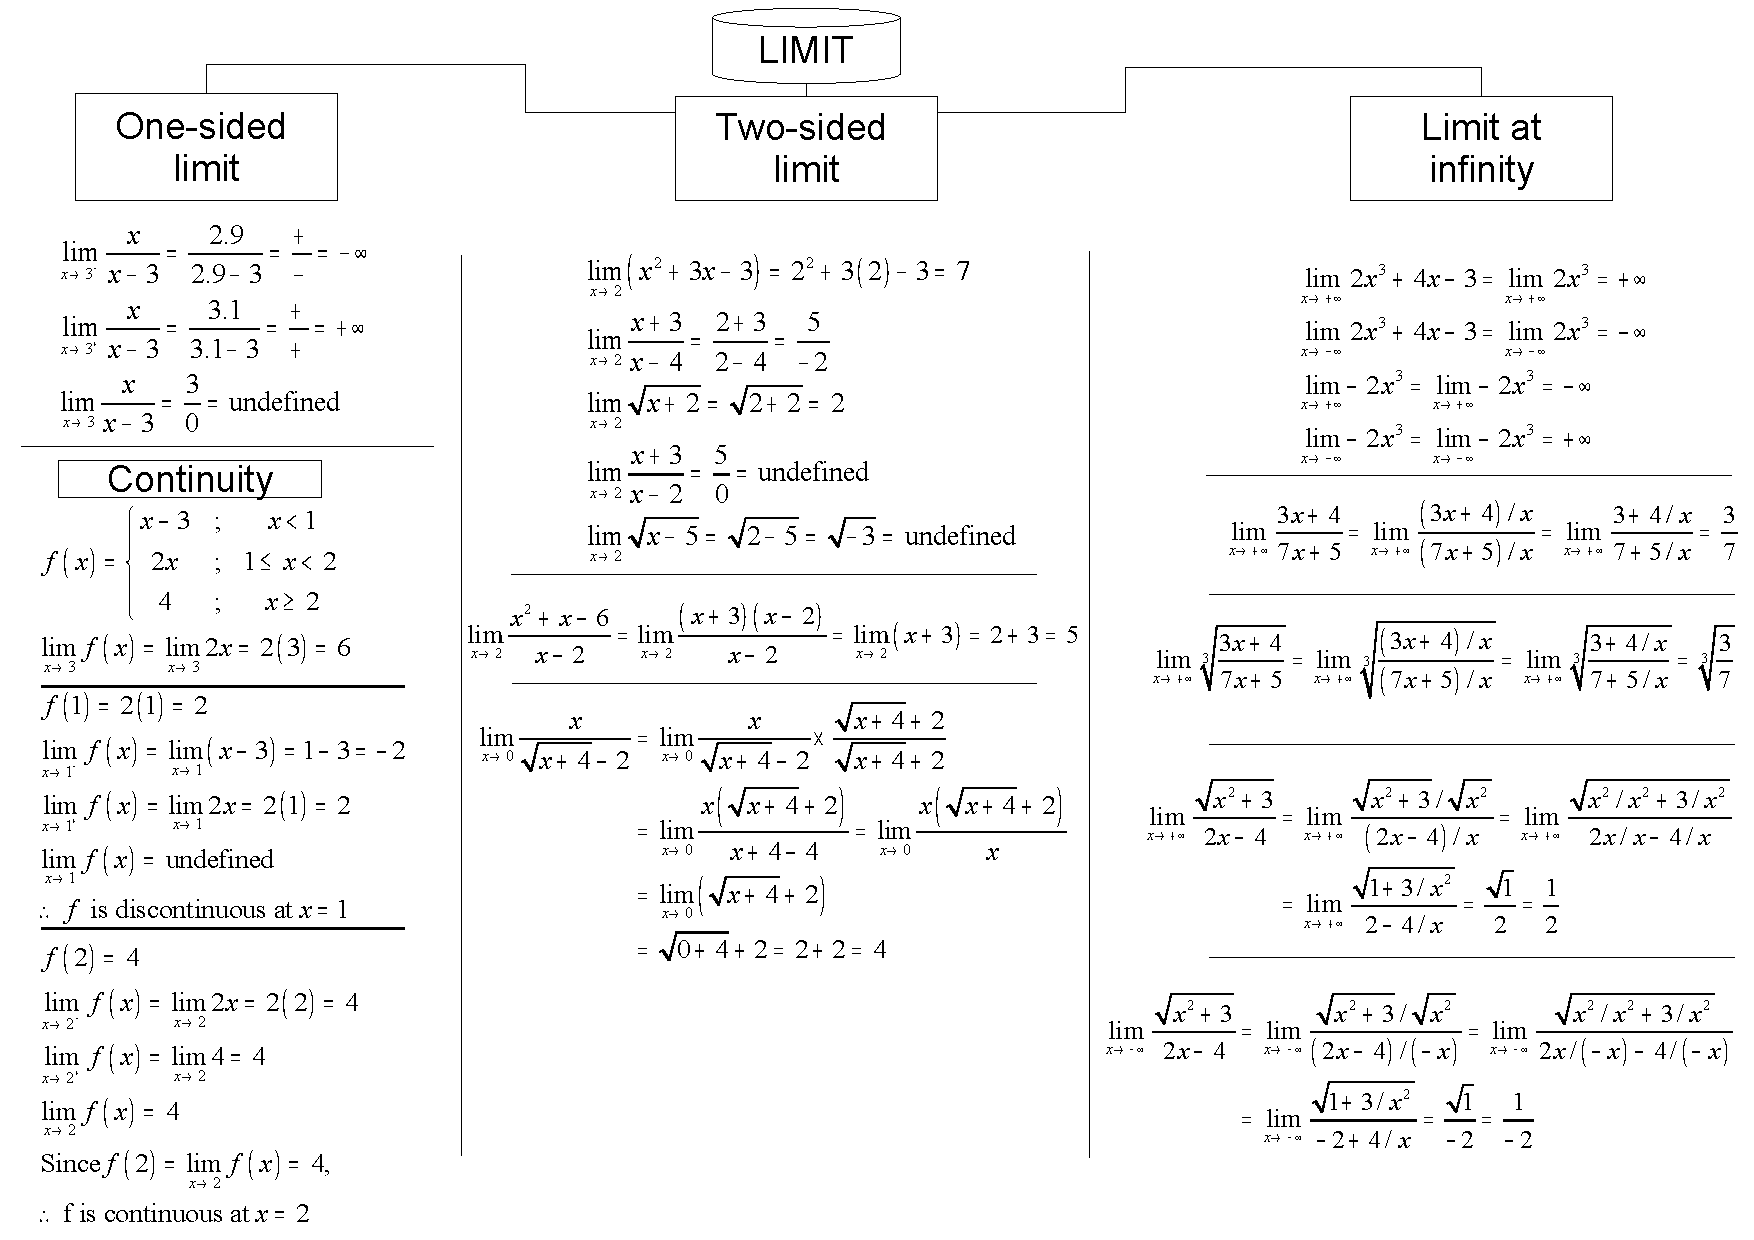
\includepdf[scale=0.7,pages={1-},angle=90,pagecommand={\chapter{Cheat Sheets}\section{Computing Limits}}]{cheat-sheets/cheat/limit}
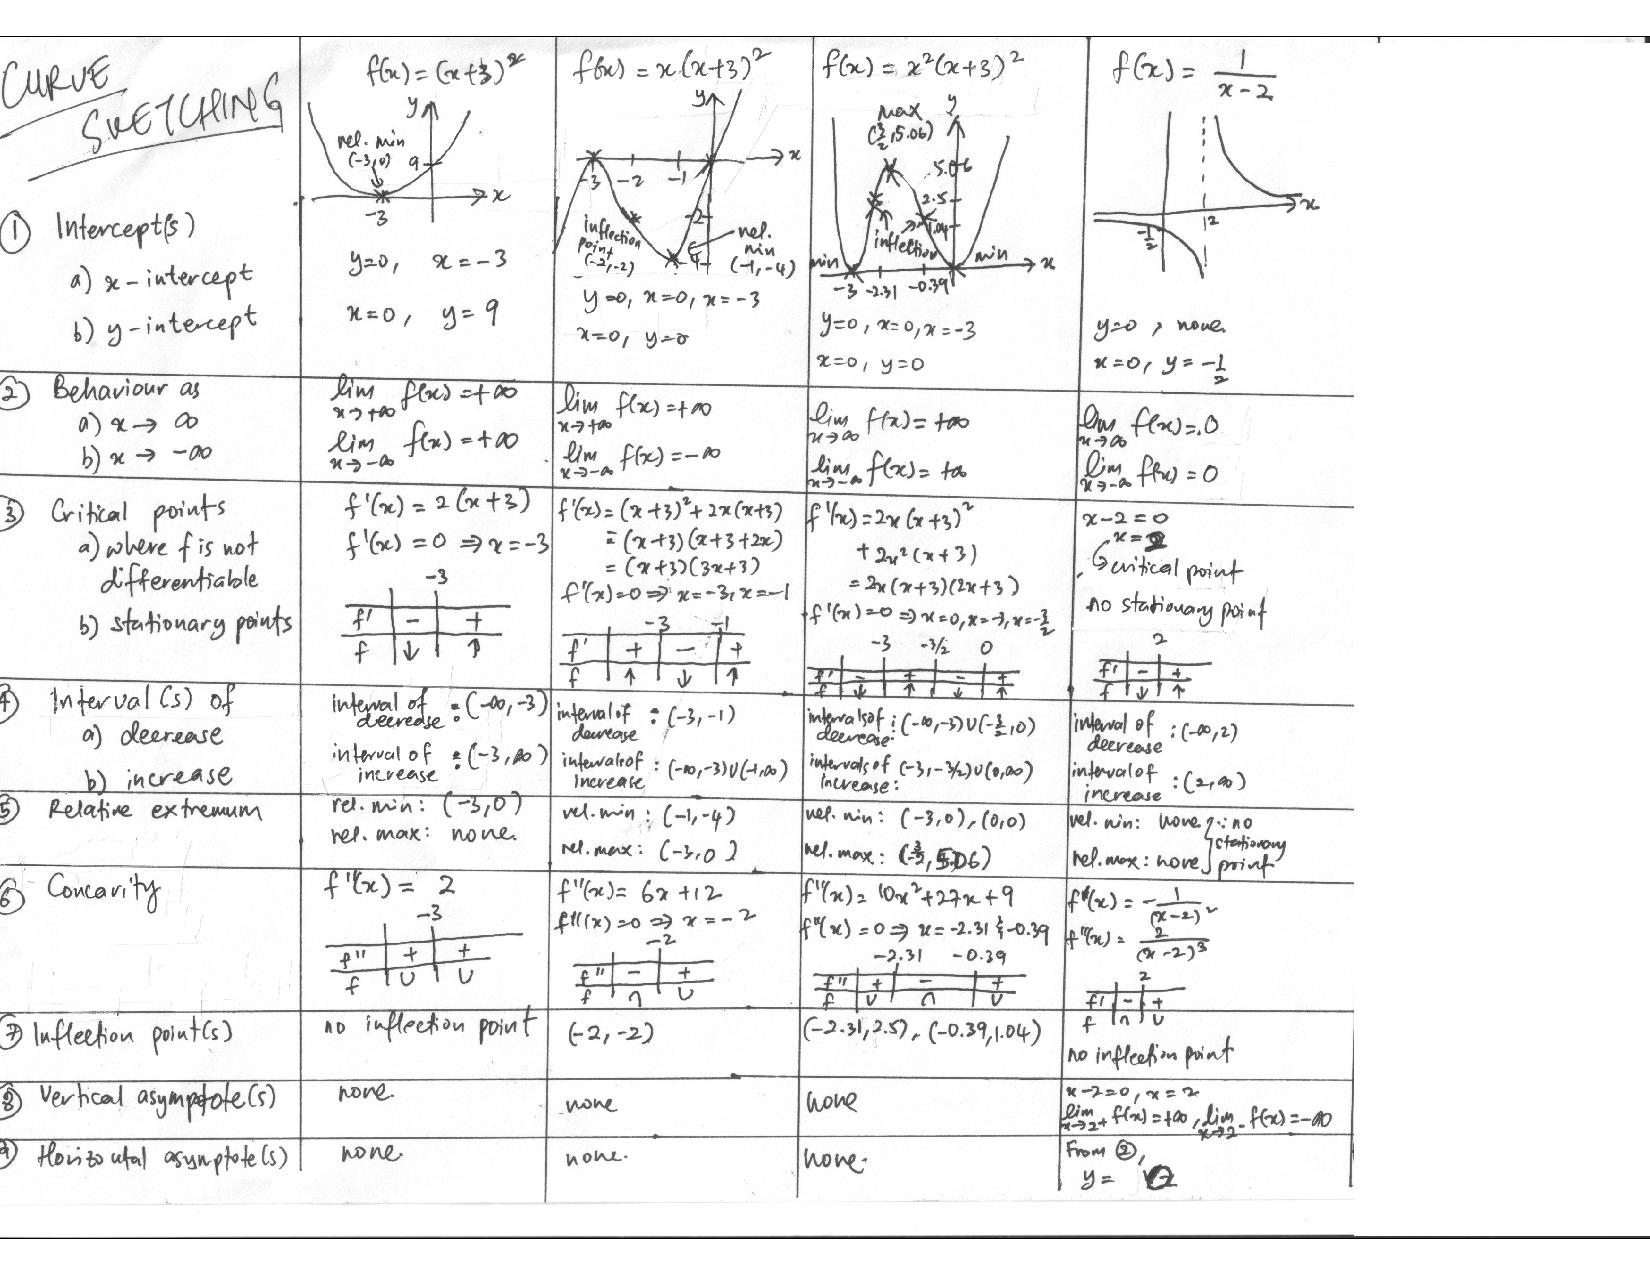
\includepdf[scale=.8,pages={-},angle=90,pagecommand={\section{Curve Sketching}}]{cheat-sheets/cheat/curveSketching}


\end{document}
